\documentclass[11pt]{article}
\usepackage[T1]{fontenc}
\usepackage[utf8]{inputenc}
\usepackage{lmodern}
\usepackage[a4paper,margin=28mm]{geometry}
\usepackage{microtype}
\usepackage{amsmath,amssymb,amsthm,mathtools}
\usepackage{enumitem,booktabs,array,graphicx,float}
\usepackage{tikz}
\usetikzlibrary{arrows.meta,positioning}
\usepackage[dvipsnames]{xcolor}
\usepackage[colorlinks=true,linkcolor=MidnightBlue,citecolor=MidnightBlue,urlcolor=MidnightBlue]{hyperref}
\usepackage[capitalise,nameinlink,noabbrev]{cleveref}
\hypersetup{pdftitle={Quaternionic division points on curves in the Siegel threefold},pdfauthor={OpenAI},pdfsubject={The quaternionic-division component of the Zilber--Pink conjecture for curves in A2}}
\newtheorem{theorem}{Theorem}[section]
\newtheorem{lemma}[theorem]{Lemma}
\newtheorem{proposition}[theorem]{Proposition}
\newtheorem{corollary}[theorem]{Corollary}
\theoremstyle{definition}
\newtheorem{definition}[theorem]{Definition}
\theoremstyle{remark}
\newtheorem{remark}[theorem]{Remark}
\newcommand{\Q}{\mathbb Q}
\newcommand{\R}{\mathbb R}
\newcommand{\C}{\mathbb C}
\newcommand{\Z}{\mathbb Z}
\newcommand{\Qbar}{\overline{\mathbb Q}}
\newcommand{\Acal}{\mathcal A}
\newcommand{\Vcal}{\mathcal V}
\newcommand{\Ecal}{\mathcal E}
\newcommand{\Ocal}{\mathcal O}
\newcommand{\id}{\mathrm{id}}
\newcommand{\dd}{\mathrm d}
\newcommand{\eps}{\varepsilon}
\newcommand{\abs}[1]{\left\lvert#1\right\rvert}
\newcommand{\norm}[1]{\left\lVert#1\right\rVert}
\newcommand{\pair}[2]{\left\langle#1,#2\right\rangle}
\newcommand{\ha}[1]{\mathrm h\!\left(#1\right)}
\newcommand{\poly}{\operatorname{poly}}
\DeclareMathOperator{\End}{End}
\DeclareMathOperator{\Hom}{Hom}
\DeclareMathOperator{\MT}{MT}
\DeclareMathOperator{\Sp}{Sp}
\DeclareMathOperator{\GSp}{GSp}
\DeclareMathOperator{\SO}{SO}
\DeclareMathOperator{\Spin}{Spin}
\DeclareMathOperator{\Gr}{Gr}
\DeclareMathOperator{\Gal}{Gal}
\DeclareMathOperator{\Tr}{Tr}
\DeclareMathOperator{\Spec}{Spec}
\DeclareMathOperator{\Supp}{Supp}
\DeclareMathOperator{\ord}{ord}
\DeclareMathOperator{\rank}{rank}
\DeclareMathOperator{\diag}{diag}
\DeclareMathOperator{\vol}{vol}
\DeclareMathOperator{\dist}{dist}
\setlist{itemsep=3pt,topsep=5pt}
\setlength{\emergencystretch}{2em}
\numberwithin{equation}{section}
\urlstyle{same}

\title{Quaternionic division points on curves\\in the Siegel threefold}
\author{OpenAI}
\date{September 24, 2026}
\makeatletter
\renewcommand{\@maketitle}{%
  \begin{center}
    {\LARGE\@title\par}
    \vspace{1.2em}
    {\large\@author\par}
    \vspace{0.6em}
    {\large\@date\par}
  \end{center}
  \vspace{1em}}
\makeatother
\begin{document}
\maketitle
\begin{abstract}
We prove the quaternionic-division component of Zilber--Pink for curves
in \(\Acal_2\) over \(\Qbar\). A Hodge-generic algebraic curve contains
only finitely many points whose full geometric rational endomorphism
algebra is an indefinite quaternion division algebra over \(\Q\).
No boundary or reduction hypothesis is required.
\end{abstract}
\begingroup
\small
\tableofcontents
\endgroup
\clearpage
\section{Introduction}\label{sec:introduction}

The Siegel moduli variety \(\Acal_2\) parametrizes principally polarized abelian surfaces and has dimension three. An indefinite quaternion division algebra can occur as the full rational endomorphism algebra of such a surface. The corresponding non-CM points lie on special curves. The Zilber--Pink conjecture predicts that a Hodge-generic algebraic curve meets the union of these special curves in only finitely many points. The quaternion algebra, its discriminant, and the endomorphism order are allowed to vary in this prediction.

For a geometric point \(s\) of \(\Acal_2\), write \((A_s,\lambda_s)\) for the represented polarized surface and put
\[
 \End^0(A_s)=\End_{\Qbar}(A_s)\otimes_{\Z}\Q.
\]
A curve is \emph{Hodge generic} if it is not contained in a proper special subvariety, including a Hecke translate of one.

\begin{theorem}\label{thm:main}
Let \(C\subset\Acal_{2,\Qbar}\) be a reduced irreducible closed Hodge-generic algebraic curve. Then
\[
 \Sigma_{\mathrm{QM}}(C)=
 \bigl\{s\in C(\Qbar):
   \End^0(A_s)\text{ is an indefinite quaternion division algebra over }\Q
 \bigr\}
\]
is finite.
\end{theorem}

Thus \Cref{thm:main} resolves affirmatively the quaternionic-division component of the Zilber--Pink conjecture for curves in \(\Acal_2\). Its condition is equality of the full geometric endomorphism algebra. In particular, it excludes the split algebra \(M_2(\Q)\) and does not replace the endomorphism condition by the existence of a quaternion embedding into a larger algebra. No condition is imposed on the boundary of \(C\), and the points are counted across all quaternionic special curves at once.

Throughout the paper, a \emph{QM point} means a point whose full geometric rational endomorphism algebra is an indefinite quaternion division algebra over \(\Q\).

\subsection{Earlier results}

The general unlikely-intersection principle asks when an intersection
with a special subvariety has larger dimension than the ambient
dimension count predicts.  Zilber formulated this principle in the
semiabelian setting \cite{Zilber2002}; Pink formulated its Shimura
counterpart \cite[Conjecture~1.3]{Pink2005}.  For a Hodge-generic curve
in a threefold, intersections with special curves have negative
expected dimension.  Pink's nondensity prediction therefore requires
finiteness even after all such special curves are allowed to vary.
The locus in \Cref{thm:main} is the part arising from division
quaternionic multiplication.

Daw and Orr proved the conclusion when the closure of the curve meets the zero-dimensional boundary stratum of the Baily--Borel compactification \cite[Theorem~1.4]{DawOrr2022}. Their reduction for an arbitrary curve assumes a large-Galois-orbit estimate \cite[Theorem~1.3 and Conjecture~6.2]{DawOrr2022}. Their later work proves finiteness against all special curves under that same boundary hypothesis \cite[Corollary~1.2]{DawOrrMultiplicative2025}. Papas obtained further finiteness results under degeneration in higher-dimensional Siegel varieties, with additional conditions on endomorphism algebras and their behavior under reduction; in dimension two, his boundary hypothesis still requires the zero-dimensional stratum \cite[Theorem~1.4]{Papas2024}.

Papas's work with \(v\)-adic values of \(G\)-functions studies neighborhoods of an interior quaternionic point. It gives a height estimate involving the number of supersingular places at which the varying point is close to the chosen center, and finiteness when that number is bounded \cite[Theorem~1.7 and Corollary~1.9]{PapasIII2025}. The horizontal good-reduction comparisons in \cite[Theorem~3.4]{PapasI2025} are also useful here. We prove a height estimate independent of the number of supersingular proximity places.

\subsection{The height argument}

Our height argument belongs to the arithmetic auxiliary-function
tradition of Bombieri and Andr\'e \cite{Bombieri1981,Andre1989}.
Interior period matrices and their $p$-adic realizations enter
Andr\'e's motivic treatment \cite{Andre1995} and Papas's work cited
above.  We prove the interpolation statement needed here directly
for fixed algebraic differential systems at an ordinary point.
In this terminology, ``ordinary'' means that the differential
system has no pole at the center; it imposes no ordinary-reduction
condition on the abelian surface.

To rule out infinitely many targets, pass to a fixed smooth fine-level cover and choose an interior quaternionic point \(t_0\). The substantive estimate is
\begin{equation}\label{eq:intro-height}
 h(t)\le c_1[K(t):K]^{c_2}
 \qquad\bigl(t\text{ a division-quaternionic point}\bigr),
\end{equation}
where \(K\) and the ample logarithmic height \(h\) are fixed. The constants may depend on the curve. This estimate is proved in \Cref{thm:height}; it is not an assumed Galois-orbit bound.

The equations come from a rank-five quadratic variation.  In the first
cohomology of each fiber, take the trace-zero operators that are
self-adjoint for the alternating polarization, with pairing
\(\pair{T}{U}=\tfrac14\Tr(TU)\).  At a QM point, the actual
Rosati-symmetric endomorphisms in this space span a positive definite
two-plane \(E_t\).  We compare a fixed pair of independent integral endomorphisms at the
center with a small integral spanning pair at the target.  Write \(B\) and
\(P\) for their de Rham coordinates, and \(Y(a)\) for horizontal
transport from the target back to the center, where \(a=x(t)\) is a
local algebraic parameter with \(x(t_0)=0\).

At places where the target is close to the center, these coordinates
satisfy a matrix of trace relations
\[
 \pair{B}{Y(a)P}=T_v\in\mathrm M_2(\Q).
\]
The four entries pair the two centered vectors with the two transported
target vectors.  At finite places the relations come from endomorphisms
of their common good reduction.  Although the rational matrix \(T_v\)
can vary with the prime, a lift of residue Frobenius fixes it.  Comparing
the relation with its conjugate therefore eliminates \(T_v\).  The two
arguments are \(a\) and \(b=aR\), where \(b\) is a conjugate of \(a\)
and \(R=b/a\) is included among the algebraic coordinates.  The number of
conjugate tuples is polynomial in the field degree, so one common system retains
a substantial sum of local smallness.  The finitely many exceptional
primes and the archimedean places are grouped directly by their trace
matrices.

The interpolation theorem in \Cref{thm:interpolation} turns this local
information into \eqref{eq:intro-height}.  Its inputs are common analytic
equations, controlled coefficient heights, sufficiently small values of
\(a\), and nonidentity on every algebraic branch used in its proof.
The auxiliary graph is obtained by adjoining the quotient of a finite
Taylor truncation of a common relation by a power of \(a\).  On this
graph, the proof constructs a low-degree polynomial.  The product
formula forces that polynomial to vanish at the target, while the
construction ensures that it does not vanish on the whole graph.
Intersection and projection then reduce the dimension of an algebraic
variety containing the target.  Repeating this descent proves the height
bound.  An ordinary-point differential estimate makes the required orders
polynomial in the algebraic degrees.

It remains to prove the nonidentity input.  Full monodromy handles the
single-argument relations and pairs of arguments that vary independently.
The exceptions are pairs lying on an isogeny correspondence dominating
both fixed curves.  There are only finitely many such correspondences,
up to integral changes of lift.  We choose one auxiliary prime \(\ell\)
and a fixed level cover on which each target admits a marking with the
following property: modulo \(\ell\), its plane and the centered plane
span a degenerate four-space.  A functional identity in the exceptional
case would force a Frobenius quasi-isogeny to act by one common sign on
both planes.  The prescribed incidence rules this out, using the
polarized multiplier and the integral trace form.  This argument also
covers supersingular reductions and target planes that are themselves
degenerate modulo \(\ell\).

Once \eqref{eq:intro-height} is known, endomorphism estimates and
one-variable Hodge-norm bounds give polynomially bounded integral
coordinates for two Hodge vectors at every point of a large Galois orbit.
The periods lie in the three-dimensional quadric of isotropic lines in
the rank-five space.  The period at a QM point is orthogonal to its
plane \(E_t\), and the orthogonal complement of each positive two-plane
cuts this quadric in a conic.  The path form of o-minimal counting would produce a one-parameter
semialgebraic family of such planes whose conics contain a nonconstant
period arc.  Their union has algebraic closure of dimension at most two.
Full monodromy, however, makes the period image Zariski dense in the
three-dimensional quadric, giving the contradiction.

This last step follows the arithmetic point-counting strategy of
Pila and Zannier \cite{PilaZannier2008}.  The rational-point theorem of
Pila and Wilkie \cite{PilaWilkie2006}, refined into definable blocks
by Pila \cite[Theorem~3.6]{Pila2011}, underlies the projected
path-counting result of Habegger and Pila
\cite[Corollary~7.2]{HabeggerPila2016} used here.  The numerical
bounds for the Hodge vectors come from the endomorphism estimates of
Masser and W\"ustholz \cite{MW1994} and Schmid's degeneration and norm
theorems \cite{Schmid1973}.  In the rank-five variation the final
geometric contradiction is a direct dimension calculation followed
by the monodromy theorem of Andr\'e \cite{Andre1992}.

\subsection{Conventions and organization}

All varieties and algebraic points are over \(\Qbar\) unless a field is specified. Algebraic heights are absolute logarithmic heights. Local absolute values extend the usual, nonsquared absolute values on \(\Q\), and local sums carry the normalized weights. The rational coordinate height used in point counting is multiplicative and will be denoted \(H_{\mathrm{rat}}\).

Constants and polynomial exponents may depend on fixed curves, covers, centers, frames, and connections. They never depend on the varying quaternion algebra or target point. A polynomial bound always refers to a fixed number of variables and fixed connection ranks.

\Cref{sec:geometry} establishes the geometric and monodromy input. The interpolation theorem is proved in \Cref{sec:interpolation}. \Cref{sec:arithmetic} constructs the arithmetic data and common equations. \Cref{sec:height} proves their nonidentity and the height estimate. \Cref{sec:counting} finishes the proof and descends to the coarse curve.

\section{The quadratic variation and its isogeny exceptions}
\label{sec:geometry}

Quaternionic multiplication will be recorded by two independent Hodge
vectors in a rank-five quadratic local system.  We first construct this
system on a fixed fine-level curve and determine its monodromy.  For two
curve arguments, failure of independent monodromy forces a polarized
isogeny relation.  We show that only finitely many such relations can
dominate the fixed curves.  This finiteness will allow the auxiliary level
in \Cref{sec:height} to be chosen before any target point is considered.

\subsection{Fixed curves and finite covers}

\begin{lemma}[Passage to fixed covers]\label{lem:finite-covers}
Let $C\subset\Acal_2$ be a reduced irreducible closed curve over $\Qbar$.
There is a finite surjective map $\pi:S\to C$ from a smooth geometrically
connected curve over a number field, together with a principally polarized abelian scheme
$f:\mathcal A\to S$ whose coarse moduli map is $\pi$.  One may obtain $S$
by normalization and a fixed full symplectic level $N\geq3$.

If infinitely many points of $C$ have the endomorphism algebra in
\Cref{thm:main}, then infinitely many points of $S$ have that property.
Deleting finitely many points of $S$, or making a further fixed finite
surjective cover and selecting a dominating connected component, preserves
this assertion.  Once all fixed data are defined over $K$, degrees and ample
logarithmic heights on the smooth completions satisfy
\begin{equation}\label{eq:fixed-cover-bounds}
 [K(\pi(t)):K]\leq[K(t):K]\leq D[K(\pi(t)):K],\qquad
 c^{-1}h_C(\pi(t))-c\leq h_S(t)\leq c h_C(\pi(t))+c,
\end{equation}
with fixed constants $D,c$.  The same statements hold for any further fixed
cover.  In particular, a degree-dependent polynomial height bound obtained
on one selected lift of every target descends to the original targets.
\end{lemma}

\begin{proof}
The full level moduli space is a fine moduli scheme with a universal abelian
scheme \cite[Chapter~I, Theorem~1.4]{Chai1985}; for the complex moduli
interpretation see also \cite[Theorem~4.6 and Corollary~4.7]{MilneModuli2013}.
The finite change-of-level group acts on it, and its quotient is the
coarse moduli space, so the forgetful map is finite.  We fix the
symplectic pairing component after adjoining the relevant roots of unity.
Normalize a component of its
pullback dominating $C$.  Normal curves in characteristic zero are smooth;
the resulting map is finite and surjective.  All the schemes and morphisms
in this construction descend to a number field.  Fibres of a finite map are
finite, so an infinite set downstairs has infinitely many lifts.  For a
cover with several components, at least one component contains infinitely
many lifts; a dominating component of a finite cover of an irreducible
curve is itself surjective.

After normalizing the base, the finite maps extend to finite maps between
smooth projective completions.  For such a map of generic degree $D_0$,
the degree formula for a fibre gives
$[K(t):K(\pi(t))]\leq D_0$.  Over the finitely many singular points of
the original coarse curve, the fixed finite map has a fixed finite set
of preimages; enlarge $D$ to bound their residue-field extensions as
well.  Thus the constant $D$ in \eqref{eq:fixed-cover-bounds} is uniform,
but need not equal the generic degree of the map to the singular curve.

Functoriality of heights identifies a height of a pulled-back ample
divisor with the height downstairs up to a bounded function.  Any two
ample divisors on a fixed projective curve bound each other's heights
linearly: sufficiently large positive integral multiples of either minus
the other are ample and have heights bounded below.  This proves
\eqref{eq:fixed-cover-bounds}.  Replacing the fixed field $K$ changes
degrees by at most a fixed factor.  None of these constants depends on the
point.
\end{proof}

Assume the target locus is infinite, as will be appropriate for the final
contradiction, and choose $S$ as in \Cref{lem:finite-covers}.  We write
$\bar S$ for its smooth projective completion.  After any required finite
deletions, choose a target $t_0\in S(\Qbar)$ and enlarge the fixed number
field $K$ so that $t_0\in S(K)$.  A rational function $x\in K(S)$ can be
chosen with a simple zero at $t_0$.  On a neighbourhood of $t_0$, it is an
\'etale parameter; its inverse germ through $t_0$ is always the germ used
below.  Other zeros of $x$ do not specify this germ.  Rational frames and
affine coordinates may be made regular on this neighbourhood by further
finite deletions away from $t_0$.  The finitely many conjugates of these
fixed data will also be treated as fixed data.  No property of the
reduction of $t_0$ is imposed here.

\subsection{A rank-five operator model}

Let $\mathbb H_{\Z}=R^1f_*\Z$ on $S(\C)$, and let $\psi$ be its alternating
polarization.  The corresponding rational local system is
$\mathbb H=\mathbb H_{\Z}\otimes\Q$.  The adjoint of an operator for $\psi$
is denoted by $T^\dagger$.  We use the weight-zero local system
\begin{equation}\label{eq:quadratic-system}
 \mathbb V=\{T\in\End(\mathbb H):T^\dagger=T,\ \Tr(T)=0\},
 \qquad \pair{T}{U}=\tfrac14\Tr(TU),\qquad q(T)=\pair{T}{T}.
\end{equation}
Its natural integral lattice is the intersection with
$\End(\mathbb H_{\Z})$.  The rational form in
\eqref{eq:quadratic-system} is integral and unimodular on this lattice
after inverting $2$.  Using another fixed commensurable integral lattice
only enlarges the finite set of excluded auxiliary primes.

\begin{lemma}[The quadratic model and the quaternionic plane]
\label{lem:qm-plane}
The local system $\mathbb V$ has rank five, a nondegenerate form of real
signature $(3,2)$, and Hodge numbers $(1,3,1)$ in types
$(1,-1),(0,0),(-1,1)$.  It is the primitive part of $R^2f_*\Q(1)$.
Conjugation of operators gives a surjective morphism of algebraic groups
\begin{equation}\label{eq:gsp-to-so}
 \rho:\GSp(\mathbb H,\psi)\longrightarrow\SO(\mathbb V,q),
 \qquad g:T\longmapsto gTg^{-1},
 \qquad \ker\rho=\mathbb G_m.
\end{equation}
Its restriction to $\Sp_4$ is the spin covering, with kernel
$\{\pm\id\}$.

At a point $t$ whose full geometric endomorphism algebra is an indefinite
quaternion division algebra, the trace-free Rosati-symmetric
endomorphisms form a rational two-plane
$E_t\subset\mathbb V_t$ of Hodge vectors.  The restriction of $q$ to $E_t$
is positive definite.  This plane is spanned by two actual integral
trace-free symmetric endomorphisms.  If $\Lambda_t=\mathbb V_{\Z,t}$, then
$L_t=E_t\cap\Lambda_t$ is saturated in $\Lambda_t$; a selected generating pair need not
generate this saturated lattice.
\end{lemma}

\begin{proof}
In a symplectic basis, the matrix of $\psi$ is
$J=\left(\begin{smallmatrix}0&I_2\\-I_2&0\end{smallmatrix}\right)$.
The equations $T^tJ=JT$ and $\Tr(T)=0$ give
\[
 T=\begin{pmatrix}A&\beta J_2\\ \gamma J_2&A^t\end{pmatrix},
 \qquad A=\begin{pmatrix}a&b\\c&-a\end{pmatrix},
 \qquad J_2=\begin{pmatrix}0&1\\-1&0\end{pmatrix}.
\]
One checks that $T^2=(a^2+bc-\beta\gamma)I_4$.  Thus
\[
 q(T)=a^2+bc-\beta\gamma,
\]
which has signature $(3,2)$ and is nondegenerate over $\Z[1/2]$.
The alternating form $(u,v)\mapsto\psi(Tu,v)$ identifies the
self-adjoint operators with alternating two-forms.  The identity operator
corresponds to $\psi$, and its orthogonal complement for the trace form
is the primitive part.  Taking account of the polarization twist gives
$\mathbb V\simeq(\bigwedge^2\mathbb H)(1)_{\mathrm{prim}}$ and the stated
Hodge numbers.

Conjugation by a similitude preserves self-adjointness and the trace
pairing.  Its determinant on $\mathbb V$ is $1$, since $\GSp_4$ is
connected.  The induced Lie algebra map
$\mathfrak{sp}_4\to\mathfrak{so}_5$ is nonzero.  Simplicity and equality
of dimensions make it an isomorphism.  Consequently the induced map on
the adjoint groups is an isomorphism; these are the split adjoint groups
of types $C_2$ and $B_2$.  Its kernel on $\GSp_4$ is exactly the scalar
torus, proving \eqref{eq:gsp-to-so} and the assertion about the spin
covering.  These statements are over $\Q$, not merely over $\C$.

Put $D=\End^0(\mathcal A_t)$.  The polarization induces the positive
Rosati involution on $D$.  Over $\R$, the identification
$D\otimes\R\simeq M_2(\R)$ turns a positive involution into the adjoint
for a positive definite form, and hence into transpose in a suitable
basis.  Its fixed subspace has dimension three.  The cohomological
trace is nonzero on the identity, so its kernel in that subspace has
dimension two.  For a nonzero symmetric endomorphism $u$, Rosati
positivity gives $\Tr(uu^\dagger)=\Tr(u^2)>0$.  Thus $q$ is positive
definite on this trace-free subspace.

The rational realization of endomorphisms on $H^1$ is faithful and
identifies endomorphisms with rational Hodge endomorphisms
\cite[Theorem~4.1]{MilneShimura1995}.  In particular
these vectors are Hodge vectors in $\mathbb V_t$.  Clearing denominators
in a rational basis gives integral endomorphisms with the same symmetry
and trace conditions.  Equivalently one can first apply
$u\mapsto u+u^\dagger$ and then
$v\mapsto4v-\Tr(v)\id$ to integral endomorphisms; the principal
polarization makes the first operation integral.  Finally, intersection
of an integral lattice with a rational subspace is saturated.
\end{proof}

Write $\Vcal_{\mathrm{dR}}$ for the algebraic de Rham realization, with its
Gauss--Manin connection and trace form.  The connection is the one
constructed from the relative de Rham complex
\cite[Theorem~1]{KatzOda1968}; its functoriality and compatibility with
cup products follow from that construction.  Algebraic--analytic de Rham
comparison \cite[Theorem~1$'$]{Grothendieck1966DeRham}, applied
to the relative complexes, identifies its horizontal local system with
the Betti realization; this relative interpretation is recorded in
\cite[Section~0.0]{Katz1970}.  Actual endomorphisms have
compatible Betti, de Rham, and \'etale realizations, and their trace
pairings are rational.  For a polarized isogeny
$\varphi:A\to A'$ with $\varphi^*\lambda'=m\lambda$, cohomological
pullback $\varphi^*:H^1(A')\to H^1(A)$ has multiplier $m$ and reverses
direction.  Our covariant transport on $H^1$ is
\[
 T_\varphi=m(\varphi^*)^{-1}:H^1(A)\longrightarrow H^1(A'),
\]
which again has multiplier $m$.  We put
$I_\varphi(u)=T_\varphi uT_\varphi^{-1}$ in the operator model.  This is
the isometry in \eqref{eq:gsp-to-so} in the direction from $A$ to $A'$;
on actual endomorphisms it realizes
$\alpha\mapsto\varphi\alpha\varphi^{-1}$.  These conventions also apply
to polarized quasi-isogenies with rational multiplier and commute with
composition.  Thus an inverse isogeny of multiplier $m$ composed with
Frobenius of multiplier $p$ has multiplier $p/m$ on this covariant
weight-one realization.  For an isogeny, $\deg\varphi=m^2$.

Under a flat trivialization, the period is the line of type $(1,-1)$ in
the smooth projective quadric
\begin{equation}\label{eq:period-quadric}
 Q_V=\{[z]\in\mathbb P(V_{\C}):q(z)=0\},\qquad \dim_{\C}Q_V=3.
\end{equation}
A rational vector is of type $(0,0)$ if and only if it is orthogonal to
this line: its reality supplies orthogonality to the conjugate line as
well.  In particular, the period at a quaternionic target is orthogonal
to $E_t$.

\subsection{Monodromy and rational isogenies}

\begin{proposition}[Single and product monodromy]\label{prop:monodromy}
For the family over any fixed smooth finite cover of a Hodge-generic
curve in $\Acal_2$, the connected algebraic monodromy on $\mathbb H$ is
$\Sp_4$, and that on $\mathbb V$ is $\SO(V,q)$.  The same holds after
pullback by a dominant morphism from an irreducible complex algebraic
variety, on a smooth open of a resolution.

Let $S_1,S_2$ be two such curves, and let an irreducible complex algebraic
variety $W$ map dominantly to both.  On the sum of the two pulled-back
weight-one systems, either the connected monodromy is
$\Sp_4\times\Sp_4$, or the image of $W$ in the product of the two moduli
curves is contained in a dominating component of a polarized isogeny
correspondence.  In the latter case the corresponding local period
relation is given by a fixed element of $\GSp_4(\Q)$ with positive
multiplier.
\end{proposition}

\begin{proof}
The generic Mumford--Tate group of a Hodge-generic curve is $\GSp_4$.
The connected monodromy normality theorem for a polarizable geometric
variation on a smooth algebraic base places connected monodromy normally
in its derived group \cite[\S5, Theorem~1]{Andre1992}.  Since $\Sp_4$ is
$\Q$-simple, the connected monodromy is either trivial or $\Sp_4$.
In the first case a finite cover kills monodromy, and the theorem of the
fixed part makes the variation constant; the moduli map would be
constant.  This is impossible.  This consequence is also recorded in
\cite[\S6, Remark~1]{Andre1992}.  A dominant pullback has the same generic
Mumford--Tate group and still has a nonconstant moduli map, so the argument
also applies there.  The assertion for $\mathbb V$ follows from
\eqref{eq:gsp-to-so}.

For the two systems let $M$ be their generic Mumford--Tate group and
$H$ their connected monodromy, after fixing rational symplectic bases
on a simply connected open.  Both projections of $H$ are $\Sp_4$.
Put $G=\operatorname{PGSp}_4$.  The algebraic Goursat lemma and simplicity
give two possibilities for the image $\bar H\subset G\times G$:
it is the product, or it is the graph of a $\Q$-defined automorphism
$\alpha$ of $G$.  Indeed the kernels of the two projections are normal;
in an adjoint simple group a proper such kernel is trivial.  In the
product case dimensions give $H=\Sp_4\times\Sp_4$.

In the graph case, every automorphism of the split adjoint group of type
$C_2$ is inner, since its Dynkin diagram has no automorphism.  As $G$ is
adjoint, a $\Q$-defined inner automorphism is conjugation by an element
$\bar g\in G(\Q)$.  The central exact sequence
\[
 1\longrightarrow\mathbb G_m\longrightarrow\GSp_4
 \longrightarrow G\longrightarrow1
\]
and $H^1(\Q,\mathbb G_m)=0$ show that $\bar g$ lifts to
$g\in\GSp_4(\Q)$.  Conjugate the second factor by this lift, so that
$\bar H$ becomes the diagonal.  Normality of $H$ in $M$ forces the
adjoint image of $M$ into the normalizer of this diagonal.  That
normalizer is the diagonal itself: a normalizing pair $(g_1,g_2)$ has
$g_2^{-1}g_1$ central in the adjoint group.

The two Hodge homomorphisms therefore agree after passage to $G$.
Their discrepancy on the weight-one spaces is a real algebraic
character of the Deligne torus
$\operatorname{Res}_{\C/\R}\mathbb G_m$ into the scalar $\mathbb G_m$.
Such a character is a power of the norm.  The two weights are equal,
so restriction to real scalars makes this power zero.  The rational
map $g$ thus identifies the Hodge structures themselves.  Its
similitude multiplier is positive because it compares the positive
definite forms supplied by their polarizations and complex structures.

This argument holds at very general points of the chosen open;
holomorphicity extends the resulting fixed period relation across it.
Write $\mu>0$ for the multiplier of
$g:H^1(A_1)\to H^1(A_2)$.  The homology map in the direction from $A_1$
to $A_2$ is
\[
 F=\mu(g^{-1})^\vee:H_1(A_1,\Q)\longrightarrow H_1(A_2,\Q).
\]
It has multiplier $\mu$ and commutes with the complex structures.
Choose an integer $n>0$ such that $nF$ is integral.  It induces a
holomorphic isogeny $\varphi:A_1\to A_2$, which is algebraic since the
tori are projective.  Its multiplier is the positive integer
$m=n^2\mu$: integrality follows by evaluating its polarization identity
on a pair of integral homology vectors of pairing $1$.
Moreover $\varphi^*=n\mu g^{-1}$, so the covariant cohomological
transport defined above is
\[
 T_\varphi=m(\varphi^*)^{-1}=ng.
\]
Thus $\varphi$ realizes the original projective rational representative.

A fixed rational similitude defines a
closed algebraic Hecke correspondence, finite over either moduli
factor.  Concretely, for a fixed integral multiplier $m$, its kernels
are among the finite subgroup schemes of $A[m]$, and the principal
polarizations and fixed level structures give the corresponding finite
moduli problem.  Closure of the local relation consequently contains
the image of $W$ in one such correspondence.  Its projections to both
curves are dominant by hypothesis.  Finite central twists of the local
systems can be killed by a finite cover and do not change this
conclusion about their moduli points.
\end{proof}

\subsection{Only finitely many dominating correspondences}

Here the finiteness concerns whole correspondences dominating two fixed
curves.  Individual isolated isogenous pairs need not belong to the
finite list.

\begin{proposition}[Finitely many isogeny exceptions]
\label{prop:finite-correspondences}
Fix finitely many closed irreducible Hodge-generic curves in
$\Acal_2(\C)$.  For every ordered pair of these curves there are finitely
many rational positive projective symplectic similitudes carrying a
lift of the first onto a lift of the second, modulo integral changes
of lifts.  Consequently all dominating polarized isogeny
correspondences between this list of curves are contained in a finite
union of closed curves in their pairwise products.  There is a fixed
finite set of positive integers $m$ such that every pair on this union
is joined by a polarized isogeny of one of these multipliers, of degree
$m^2$.  Refining the fixed level does not enlarge the required set of
underlying multipliers.
\end{proposition}

\begin{proof}
We first show that the real stabilizer of a lifted curve is discrete.
Finite area of the curve quotient will then make its integral stabilizer
a subgroup of finite index.  Maps between two lifts consequently have
only finitely many cosets, and rational representatives will give the
fixed isogeny multipliers.

Let $\mathfrak H_2$ be Siegel space, let
$G_{\R}=\operatorname{PGSp}_4(\R)^+$ be its effective connected group of
holomorphic isometries, and fix a torsion-free principal congruence
subgroup $\Gamma$ at fine level.  For any curve in the list, choose an
irreducible analytic component $X$ of its full inverse image in
$\mathfrak H_2$.  It is a closed analytic curve.  Its normalization
may be used wherever a smooth curve is needed.  The integral stabilizer
\[
 \Gamma_X=\{\gamma\in\Gamma:\gamma X=X\}
\]
contains the image of the monodromy of the normalization of the
corresponding fine-level curve.  In fact this image is the deck group
on the lifted normalization over the smooth part.  By
\Cref{prop:monodromy}, it is Zariski dense in the real adjoint group.

We verify that the real stabilizer
\[
 H_X=\{g\in G_{\R}:gX=X\}
\]
is discrete.  It is closed: if $g_n\to g$ with $g_nX=X$, closedness of
$X$ gives $gX\subset X$, and applying the same argument to $g_n^{-1}$
gives equality.  Thus $H_X$ is a Lie subgroup.  Its Lie algebra is
invariant under $\Gamma_X$.  Stabilizing a fixed real vector subspace
of the adjoint representation is an algebraic condition, so Zariski
density makes this Lie algebra an ideal of
$\mathfrak{sp}_4(\R)$.  Simplicity leaves zero or the full Lie algebra.
The latter would give $H_X=G_{\R}$, forcing $X=\mathfrak H_2$ by
transitivity.  The dimensions differ, so $H_X$ is discrete.

Discreteness alone does not bound the number of cosets of $\Gamma_X$.
For this we use that $\Gamma_X\backslash X$, with normalization understood,
has finite area for the metric induced from an invariant Hermitian
metric on $\mathfrak H_2$.  To check both the quotient and the effect
of singularities, let $S_X$ be the normalization of the corresponding
closed fine-level curve and form
\[
 Y=S_X\mathbin{\times}_{\Gamma\backslash\mathfrak H_2}\mathfrak H_2.
\]
The normalization map from $S_X$ to its closed fine-level image is
finite, so base change makes $Y\to\mathfrak H_2$ finite, with image
the full inverse image of that curve.  On the other hand,
$Y\to S_X$ is a covering and locally a biholomorphism, so $Y$ is
smooth.  The finite map to that inverse image is an isomorphism above
the smooth locus of the curve; hence it is its normalization.

The component $Y_0$ normalizing $X$ has stabilizer
$\Gamma_X$; this group acts transitively on every fibre over $S_X$, since a deck
transformation carrying two points of the same fibre to one another
preserves their common connected component, and
$\Gamma_X\backslash Y_0\simeq S_X$.  It therefore suffices to bound the
pullback metric at the finitely many punctures of $S_X$.

For completeness, any holomorphic map from the unit disk to
$\mathfrak H_2$ contracts its invariant metric up to a fixed constant
relative to the Poincar\'e metric.  Realize $\mathfrak H_2$ as a bounded
domain.  An automorphism moving the image of the origin to a fixed
origin, followed by the Cauchy derivative estimate in bounded
coordinates, bounds the derivative at zero uniformly.  Disk
automorphisms give the pointwise assertion.  Apply it on the universal
cover of a punctured parameter disk.  The descended upper bound is a
constant multiple of
\[
 \frac{|du|^2}{|u|^2\log^2(1/|u|)},
\]
whose area on $0<|u|<\varepsilon$ is finite.  On the remaining compact
part the period map is holomorphic and has finite area.  Zeros of its
derivative or singular branches only decrease this upper bound.

We now deduce the precise group-theoretic consequence
\begin{equation}\label{eq:stabilizer-index}
 [H_X:\Gamma_X]<\infty.
\end{equation}
The action of $G_{\R}$ on $\mathfrak H_2=G_{\R}/K_{\mathrm{max}}$ is
proper, since $K_{\mathrm{max}}$ is compact.  Therefore the discrete
group $H_X$ acts properly on $X$, with finite point stabilizers.  Choose
a regular point $z\in X$ and a sufficiently small $H_{X,z}$-invariant
disk $D\subset X$ of positive induced area such that $gD\cap D$ is
empty for $g\notin H_{X,z}$.  Distinct double cosets in
$\Gamma_X\backslash H_X/H_{X,z}$ give disjoint images of translates of
$D$ in $\Gamma_X\backslash X$.  Each translate embeds there: a further
identification would give a nonidentity element of the torsion-free
group $\Gamma_X$ conjugate to an element of the finite group $H_{X,z}$.
All these disks have the same positive area.  Finite total area thus
bounds the number of double cosets, and finiteness of $H_{X,z}$ bounds
the number of left cosets.  This proves \eqref{eq:stabilizer-index}.

Choose lifts $X_1,X_2$ for two curves.  If a rational positive projective
similitude $g_0$ carries $X_1$ onto $X_2$, the set of all real such
maps is $g_0H_{X_1}$.  By \eqref{eq:stabilizer-index} this set has only
finitely many classes modulo right multiplication by
$\Gamma_{X_1}$.  Every class containing a rational map admits a rational
representative.  Integral changes of the chosen lifts add no classes:
at coarse level all lifts are conjugate under the full integral
symplectic group; at the chosen fine level there are only finitely
many resulting classes.  Thus there are finitely many rational maps
for the whole fixed list.

A dominating component of a Hecke correspondence determines a local
equality between a rational translate of one lifted curve and another
lifted curve.  Both are irreducible closed analytic curves, so this
local equality extends to equality of those lifts.  It is therefore
represented by one of the finite maps just obtained.  Lift each
projective rational representative to $\GSp_4(\Q)$, using
$H^1(\Q,\mathbb G_m)=0$, and clear denominators on the integral homology
lattices.  Its multiplier becomes a positive integer $m$.  This gives an isogeny of multiplier $m$ on the local correspondence.
To retain that multiplier after taking closure, work over the fixed
fine moduli space in characteristic zero.  Subgroups
$K\subset A[m]$ that are maximal isotropic for the Weil pairing and
have order $m^2$ form a finite \'etale scheme over this space:
\'etale-locally the torsion is a constant finite group.  Each such
subgroup gives the quotient $B=A/K$ with its principal polarization
characterized by $q^*\lambda_B=m\lambda_A$.  The resulting map to
$\Acal_2\times\Acal_2$ is finite.  Indeed it is finite over the first
coarse factor, hence proper into the product because the second
factor is separated, and its fibres are finite.  Its image is
therefore closed, and every geometric point of that image admits an
isogeny of multiplier $m$.  The closure of the local correspondence
lies in this image, including at singular coarse points and points
with extra automorphisms.

Taking all representatives and the finitely many curve components of
their intersections with the pairwise products that dominate both factors
gives the required finite union.  Additional level structures change only
the finite covers of these moduli problems, not the underlying
isogenies or their multipliers.
\end{proof}

We apply \Cref{prop:finite-correspondences} to the full finite list of
absolute Galois conjugates of the original closed coarse curve $C$.
The canonical Siegel moduli space has reflex field $\Q$, and Galois
conjugation permutes its special subvarieties
\cite[Corollary~5.3, arXiv version~2]{Orr2021}.  If a conjugate of $C$ lay in a proper
special subvariety, inverse conjugation would contradict the Hodge
genericity of $C$.  Thus every curve in this list is Hodge generic.
Enlarging $K$ for centers or markings adds no coarse image to this
list.  The resulting finite set of multipliers, the chosen center,
and the rank-five lattices are fixed before the prime $\ell$ and the
marking cover of \Cref{prop:marking} are selected.  Refining level changes
the markings over these same coarse images; the exceptional isogenies
are required only between the underlying polarized abelian varieties.
Later estimates may therefore be proved on that fixed cover and
descended by \Cref{lem:finite-covers}.

\section{Interpolation with two arguments}\label{sec:interpolation}

This section proves a polynomial height bound from common analytic
relations at a weighted collection of places.  The relations involve a
small algebraic parameter $a$, auxiliary algebraic coordinates $U$, and
solutions of fixed ordinary differential systems.  A second argument may
be $aR$, where $R$ is a coordinate of $U$.  The conclusion will bound a
height parameter $h$ polynomially in a complexity parameter $d$, provided
the relations are not all identities on any of the algebraic branches
used in a dimension descent.

\subsection{Weighted absolute heights}

For a tuple $z=(z_i)$ over a number field $F$, write
$\norm z_v=\max_i|z_i|_v$ and put
\[
 \ha{z}=\sum_v w_v\log\max(1,\norm{z}_v),
 \qquad w_v=\frac{[F_v:\Q_v]}{[F:\Q]}.
\]
At the infinite places the absolute value is the usual, unsquared one;
thus a complex place has weight $2/[F:\Q]$.  The same notation for a
polynomial, or a finite list of polynomials, means the height of its
complete coefficient tuple \emph{with the additional coordinate $1$}.
It therefore bounds the scale of the coefficients.  For each fixed
number of variables,
\begin{equation}\label{eq:polynomial-evaluation}
 \log\abs{G(z)}_v
 \leq \log\max(1,\norm{\operatorname{coeff}G}_v)
       +\deg(G)\log\max(1,\norm z_v)
       +\eps_v\log\#\operatorname{mon}(G),
\end{equation}
where $\eps_v$ is $1$ at an infinite place and $0$ otherwise.
In particular, the sum of the last terms is controlled without counting
the finite places.

Occasionally the selected local data distinguish embeddings inducing the
same place.  We then use embeddings $F\hookrightarrow\C$ or
$F\hookrightarrow\C_p$, each with weight $1/[F:\Q]$, which gives the
same height formula.  A selection of embeddings is allowed.  On replacing
$F$ by a finite extension, we always take \emph{all} extensions of each
selected embedding.  The sum of their weights is its original weight.
All selected sums below are consequently unchanged by such an extension.
No bound for the degree of a normal closure or of an auxiliary coefficient
field will be used.

\subsection{The interpolation statement}

In the statement, the finite list of curves, connections, ordinary
centres, rational frames regular at the centres, and algebraic chart
germs is fixed.  Its ranks and all polynomial-combination degrees are
fixed.  An allowed analytic expression is a polynomial combination of
the algebraic coordinates $(a,U)$, these chart germs, and entries of the
horizontal solution matrices, evaluated at $a$ and possibly at $aR$,
where $R$ is one of the coordinates of $U$.  Constant summands are
allowed.  The total degree in all polynomial factors, including $a$
and every coordinate of $U$, is bounded by a fixed constant.  Only
substitution into the fixed germs produces Taylor coefficients of
growing degree.  The scalar coefficients of the combination may be
algebraic and vary with the target.

\begin{theorem}[Common-relation interpolation]\label{thm:interpolation}
Fix the analytic data just described, a fixed affine ambient space with
coordinates $(a,U)$, and an algebraic ambient locus $X$ in that space.
Let $h,d\geq2$, let $\Psi(h)=1+(\log h)^c$ for a fixed $c\geq1$, and
let $z_*=(a_*,U_*)\in X(\Qbar)$ with $a_*\ne0$.  Suppose that the
following bounds hold, with fixed polynomials $Q_i$ having nonnegative
coefficients.
\begin{enumerate}[label=\textup{(\roman*)}]
\item The ambient locus has equations of degree at most $Q_0(d)$ and
affine height at most $Q_0(d)\Psi(h)$, and
$\ha{z_*}\leq Q_0(d)h$.
\item There is a finite weighted selection $\mathcal V$ of places or
embeddings for which $\abs{a_*}_v<1$ and
\begin{equation}\label{eq:interpolation-smallness}
 S_{\rm small}:=\sum_{v\in\mathcal V}w_v
               \log\frac1{\abs{a_*}_v}
 \geq\frac{h}{Q_1(d)},\qquad
 \sum_{v\in\mathcal V}w_v\log\max(1,\norm{U_*}_v)
 \leq Q_2(d)\Psi(h).
\end{equation}
If the second argument occurs, $\abs{R_*}_v=1$ for these local data.
\item A common list of fixed length $s$ of allowed expressions
\[
 E_\nu(a,U)=\sum_{j\geq0}a^j e_{\nu j}(U),\qquad 1\leq\nu\leq s,
\]
vanishes at $z_*$ at every selected local datum.  Its coefficients satisfy
\[
 \deg e_{\nu j}\leq C(1+j),\qquad
 \ha{(e_{\nu j})_{\nu,\,0\leq j\leq l}}
 \leq Q_3(l,d)\Psi(h).
\]
There are $b_v\geq0$ with
$\sum_{v\in\mathcal V}w_v b_v\leq Q_4(d)\Psi(h)$ such that the
convergent tails at the target satisfy, for every $l\geq0$,
\begin{equation}\label{eq:interpolation-tail}
 \left|\sum_{j\geq l}a_*^j e_{\nu j}(U_*)\right|_v
 \leq \abs{a_*}_v^l\exp((1+l)b_v).
\end{equation}
\item If $W\subseteq X$ is an irreducible algebraic variety containing
$z_*$ on which $a$ is nonconstant, then on every normalization branch
above the generic point of every component of $W\cap V(a)$ the
expressions $E_1,\ldots,E_s$ are not all identically zero.  The
expressions use their specified ordinary chart germs.
\end{enumerate}
Then $h\leq C_1d^{C_2}$, with constants depending only on the fixed data
and the polynomials in the hypotheses.
\end{theorem}

The hypothesis in (iv) includes branches on proper subvarieties of $X$.
The proof only uses the varieties encountered in the descent below, so
verification on those varieties suffices.  In the application this is
the role of \Cref{prop:nonidentity}.

Here is the descent mechanism.  Suppose that $h$ is larger than a
polynomial in $d$, and let $W\subseteq X$ be an irreducible variety
containing the target.  When $a$ is nonconstant and $W$ meets $a=0$,
we pass to a graph $W'$ that is isomorphic to $W$ over $a\ne0$.
On this graph we construct a polynomial $P$ with
\[
 P\notin I(W'),\qquad P(z_*')=0,
\]
where $z_*'$ is the lifted target.  The intersection with $P=0$ then
projects to a smaller-dimensional variety containing $z_*$.  We discard
the graph coordinate after each step, so the ambient dimension stays
fixed.

The two requirements on $P$ have different sources.  Nonidentity in
(iv), together with an ordinary-point zero estimate, gives a graph whose
special fibre satisfies a codimension-two condition after one further
equation is imposed.  Counting coefficients layer by layer in powers of
$a$ then gives a polynomial nonzero on $W'$ whose target value is bounded
locally by $|a_*|_v^n$ times controlled factors.  The ratio of $n$ to its
degree $L$ can exceed any prescribed polynomial in $d$, while both $n$
and $L$ remain polynomially bounded.  At the selected places, the factor
$|a_*|_v^n$ contributes $-nS_{\rm small}$ to the logarithm of its value.
At the other places, its degree costs at most $L$ times the global height
of the lifted target.  For a sufficiently large ratio
$n/L$, the product formula forces $P(z_*')=0$.  The remaining errors
are polynomial multiples of $\Psi(h)$ and are absorbed when $h$ is large.

\subsection{Effective algebra in fixed dimension}

The descent needs two kinds of algebraic bounds: equations for each
smaller variety must retain controlled degree and height, and the
interpolation polynomial must have a membership identity with controlled
coefficients.  We record both bounds here.  Throughout this subsection,
``controlled'' means polynomial in the input degrees and linear in
$1+$ the joint logarithmic coefficient height, with ambient dimension
fixed.

In a fixed number of variables, ideals with generators of degree at most $D$ have
Gr\"obner bases of degree polynomial in $D$, for any prescribed monomial
order \cite[Corollary~8.3]{Dube1990}.  We may first discard generators
linearly dependent on the others, leaving polynomially many.  If a
polynomial belongs to such an
ideal, the degrees in a membership representation are polynomial in
$D$ and the degree of that polynomial
\cite[Theorem~3.4]{Aschenbrenner2004}.  This is a bound for arbitrary
ideal membership.

These degree bounds also give coefficient bounds from the original
input coefficients.  Let $\delta$ be the Gr\"obner-basis degree bound,
and choose the minimal monomial generators $M_\alpha$ of the initial
ideal.  Each is the leading monomial of a polynomial of degree at most
$\delta$ in the ideal.  Seek such a polynomial in the form
\[
 H_\alpha=M_\alpha+
 \sum_{\substack{N<M_\alpha\\\deg N\leq\delta}}c_{\alpha N}N,
 \qquad H_\alpha=\sum_i A_{\alpha i}G_i.
\]
The membership bound supplies a polynomial bound for the degrees of
the $A_{\alpha i}$.  The displayed coefficient equations are therefore
a solvable affine linear system of polynomial size whose entries are
only the original coefficients and $0,\pm1$.  A solution obtained by
nonzero minors bounds the coefficients of $H_\alpha$ and its
representation simultaneously.  The resulting $H_\alpha$ form a
Gr\"obner basis, since their leading monomials generate the initial
ideal.  Thus no bound for coefficients of a previously chosen basis
is presumed.

If the joint affine height of the input is $H$, a determinant of size
$s$ has height at most $sH+s\log s$.  Normalizing a nonzero coordinate
and concatenating polynomially many coefficient lists incurs only a
polynomial factor.  Consequently all these affine coefficient heights
are at most $Q(D)(H+1)$: the dependence on the logarithmic input height
is linear.  The same argument treats elimination and saturation; for
example saturation by $a$ is computed by eliminating $z$ after
adjoining $za-1$.

For varieties, the degree and arithmetic B\'ezout inequalities give the
following consequence: intersections, closures of coordinate projections,
and choices of irreducible components have degrees polynomial in the
input degrees and Chow heights at most a polynomial in the input degrees times $1+$
the joint input height.  Here and below the ambient dimensions are fixed.
We use the arithmetic B\'ezout inequality
\cite[Corollary~2.11]{KPS2001}, the projection bound
\cite[Lemma~2.6]{KPS2001}, and additivity and nonnegativity of cycle
heights \cite[Section~1.2.4]{KPS2001}.  The comparison of Chow
coefficient height with this cycle height is
\cite[Lemma~1.1, inequality~(1.2), and Section~1.2.4]{KPS2001}.
One may work throughout with Chow forms, normalizing one nonzero
coefficient to $1$.  The affine height of the normalized coefficient
tuple then equals its projective height, by the product formula.

It is enough to recover equations \emph{set-theoretically} from a Chow
form.  Indeed, if $Z\subset\mathbb P^N$ has dimension $r$ and Chow form
$\mathcal C_Z$, substitute the $r+1$ hyperplanes
\[
 \sum_{j=1}^N T_{ij}(X_j-x_jX_0)=0\qquad(0\leq i\leq r)
\]
in $\mathcal C_Z$ and take its coefficients as a polynomial in the
$T_{ij}$.  These coefficients vanish at $x$ precisely when
$[1:x]\in Z$: outside $Z$, the hyperplanes through that point form a
base-point-free system on $Z$, and $r+1$ general members have empty
intersection on $Z$.  The resulting equations have degree at most
$(r+1)\deg Z$ and controlled affine coefficient heights by expansion.
Their number is polynomial in $\deg Z$.

Thus every variety used below admits an ideal $\mathfrak b$ of controlled
generators with
\begin{equation}\label{eq:controlled-support}
 V(\mathfrak b)=W,\qquad \mathfrak b\subseteq I(W).
\end{equation}
We need not compute generators of the radical $I(W)$.  The distinction
will be useful: ideal membership in $\mathfrak b$ suffices for evaluation
on $W$, while nonvanishing on $W$ will be imposed separately.

\subsection{An ordinary-point zero estimate}

The differential method compares successive derivatives in a
finite-dimensional row space; see the classical multiplicity estimate
of Bertrand and Beukers \cite[Theorem~1]{BertrandBeukers1985}.
We give the argument here because the algebraic variety on which the
system is restricted varies in the descent, and the bound must be
polynomial in its degree while allowing the second argument $aR$.

\begin{lemma}[Uniform ordinary-point order bound]\label{lem:zero-estimate}
For the fixed analytic data of \Cref{thm:interpolation} there is a
polynomial $M(D)$ with the following property.  Let $W$ be an irreducible
affine variety of degree at most $D$ on which $a$ is nonconstant.  On a
branch above the generic point of a component of $V_W(a)$, every allowed
expression $E$ which is not identically zero satisfies
\begin{equation}\label{eq:divisorial-zero-estimate}
 \operatorname{ord}_{\mathfrak p}E
 <M(D)\operatorname{ord}_{\mathfrak p}a.
\end{equation}
The bound is independent of the heights of the coefficients of $W$ and
of the expression.
\end{lemma}

\begin{proof}
We first preserve the branch order on a curve of controlled degree, then
use the ordinary differential equation to bound that order independently
of coefficient heights.

\emph{Reduction to a curve.}  Write $k=\dim W$, and
let $\widetilde D$ be the normalization divisor defining the branch.
At a general point $p$ of $\widetilde D$, both the normalization and
$\widetilde D$ are smooth, and the finite map from $\widetilde D$ to
its image $D_0$ is \'etale at $p$ after restricting to dense open
subsets, by separability in characteristic zero.  Choose $k-1$ general affine linear functions
whose differentials restrict to a basis of the cotangent space of
$D_0$ at the image of $p$.  Their pullbacks restrict to a basis on
$\widetilde D$.  Their common level set through $p$ is consequently
a smooth curve germ transverse to $\widetilde D$ in the normalization.
The downstairs linear section is proper and has total projective
degree at most $D$.  The transverse germ leaves the nonnormal locus,
so its map to its image curve is generically the normalization
isomorphism.  It is thus the corresponding smooth germ on the
normalization of an irreducible component of that linear section.

This slice preserves formal orders as well.  If
$\operatorname{ord}_{\widetilde D}a=e>0$ and
$\operatorname{ord}_{\widetilde D}E=N$, only the terms with $j\leq N/e$
contribute to the leading coefficient.  After deleting a proper closed
subset of $\widetilde D$, write $a=t^ev$ and that finite truncation as
$t^Nu$, where $t$ is a local equation of $\widetilde D$ and $u,v$ are
units.  On the transverse curve $t$ is a uniformizer.  Hence the
orders are exactly $e$ and $N$ after restriction.  All these conditions
hold at a general slice point.

Let $T_0$ be the smooth projective normalization of this sliced curve.
Its genus is polynomial in $D$, by a general birational plane
projection and the arithmetic genus of a plane curve.  Every ambient
coordinate on $T_0$ is a quotient $X_i/X_0$, so its polar divisor has
degree at most $D$.  In particular the maps defined by $a$ and $aR$
have degrees at most $D$ and $2D$, respectively.

Adjoin the points on the fixed curves specified by the algebraic chart
germs.  Constant argument maps contribute constant chart factors and
require no cover; in what follows index only the nonconstant argument
maps.  If the corresponding fixed maps to $\mathbb P^1$ have degrees $d_i$ and
branch sets $B_i$, including infinity when it is a branch value, the
chosen normalized fibre-product component $T\to T_0$ has degree at
most $N_0=\prod_i d_i$.  It is \'etale outside
$\bigcup_i\phi_i^{-1}(B_i)$, where $\phi_i$ is $a$ or $aR$.
This set has at most $\sum_i\#B_i\deg\phi_i=O(D)$ points, and the
ramification contribution above each is at most $N_0$.  Thus
Riemann--Hurwitz gives
\[
 2g(T)-2\leq N_0\max\{0,2g(T_0)-2\}+O(D).
\]
The degrees of the maps
from $T$ to the fixed curves are bounded by $N_0\deg\phi_i$, so all
pulled-back fixed divisors have polynomial degree.  Poles of $aR$ are
included in this calculation through the fibre above infinity.  All
ramification indices are bounded as well; any further ramification
multiplies the two orders in
\eqref{eq:divisorial-zero-estimate} by the same factor.

\emph{The ordinary differential system.}  Let $p\in T$ be the point of
the specified branch.  In direct sums and tensor products of the fixed
pulled-back systems the expression takes the form
\[
 E=r_0y,
\]
where $y$ is a horizontal column of a fixed rank $N$ and $r_0$ is a
rational row.  Polynomial algebraic factors are absorbed in $r_0$.
A constant map to one of the fixed curves contributes a constant
horizontal factor.  The rational frames here are the pullbacks of the
fixed frames; they are regular and invertible at $p$.  In fact $a=0$
and $R$ is regular at the chosen affine divisor, so both arguments
$a$ and $aR$ are at their ordinary centres.  The connection and $r_0$
are therefore regular at $p$.  Their global polar divisors have degrees
polynomial in $D$, by the bounds on the degrees of the pullback maps
and of the coordinate functions.

Choose a rational function $z$ on $T$ which is a uniformizer at $p$ and
whose polar divisor has degree at most $2g(T)+1$.  Such a function follows
from Riemann--Roch by prescribing its first two jets at $p$ and allowing
a pole at another point.  For $g(T)=0$ a degree-one function suffices.
Put $\delta=d/dz$, and write the horizontal equation as $\delta y=Ay$.
The poles of the rational vector field $\delta$ are bounded in degree by
the zero divisor of $\dd z$, hence by $2g(T)-2+2\deg z$.  Differentiating
a rational function adds at most its reduced polar divisor and the
polar divisor of this vector field.  It follows that $A$, $r_0$, and
any fixed number of their derivatives have polar degrees polynomial in
$D$.  They remain regular at $p$; using a uniformizer rather than
dividing by $\dd a$ accommodates arbitrary ramification of $a$.

Set
\[
 r_{i+1}=\delta r_i+r_iA.
\]
Then $\delta^iE=r_iy$.  The successive rows become dependent after at
most $N$ steps.  If $r_\rho$ is the first row dependent on its
predecessors, their span
$M=\langle r_0,\ldots,r_{\rho-1}\rangle_{\C(T)}$ is stable under the
dual connection: differentiating the dependence shows that every later
row belongs to it.  Here $\rho\leq N$.

Let $\mathcal O=\mathcal O_{T,p}$ and saturate the common kernel of
these rows in $\mathcal O^N$.  Saturation makes it a subbundle locally.
It is stable under the ordinary connection, since its derivative is
regular and belongs to the kernel generically.  The quotient has an
ordinary connection as well.  Explicitly, if $v$ is a local section
annihilated by every row in $M$, stability of $M$ under the dual
connection gives $r(\nabla_\delta v)=0$ for every $r\in M$.
The ordinary connection makes $\nabla_\delta v$ regular, so it belongs
to the saturated kernel.  The kernel and its quotient are free over
the local discrete valuation ring, and the induced quotient connection
has no pole.  The image $\bar y$ of $y$ in this
quotient is a nonzero horizontal section: a zero image would give
$r_0y=E=0$.  Conversely, if $E$ were identically zero, all its
derivatives $r_i y$ would be zero and $y$ would lie in the kernel.
The nonzero horizontal quotient section has
nonzero reduction at $p$: the coefficient recurrence of an ordinary
linear differential equation forces a horizontal section with zero
initial value to be zero.

The integral dual of this free quotient is exactly the saturated row
lattice $\mathcal L=M\cap\mathcal O^N$: its rows are the integral
functionals annihilating the common kernel.  Since $\bar y$ has nonzero
reduction, one such functional $\lambda\in\mathcal L$ has
$\lambda y$ a unit.  Choose a nonzero $\rho\times\rho$ minor $\Delta$
of the matrix with rows $r_0,\ldots,r_{\rho-1}$.  All these rows are
regular at $p$.  Cramer's rule on the selected columns gives
\[
 \Delta\lambda=\sum_{i=0}^{\rho-1}c_ir_i,
 \qquad c_i\in\mathcal O.
\]
Hence at least one $i<\rho$ satisfies
$\operatorname{ord}_p(r_iy)\leq\operatorname{ord}_p\Delta$.
This is the elementary-divisor bound for the row lattice, expressed
without choosing a new global frame.  A nonzero rational function on
$T$ has equal total zero and pole degrees, so
$\operatorname{ord}_p\Delta$ is bounded by its polar degree, which is
polynomial in $D$.  Finally, since $z$ is a uniformizer,
\[
 \operatorname{ord}_p E
 \leq\operatorname{ord}_p(\delta^iE)+i
 \leq\operatorname{ord}_p\Delta+N-1.
\]
Increasing the resulting polynomial by $1$ proves
\eqref{eq:divisorial-zero-estimate}, since
$\operatorname{ord}_p a\geq1$.  This construction used only degrees,
genera, ramification and fixed ranks; it used no arithmetic height.
\end{proof}

\subsection{The graph and its special fibre}

\begin{lemma}[Dimension of the constrained graph fibre]\label{lem:graph-fiber}
Let $W$ be an irreducible affine variety of dimension $k\geq1$ with
coordinate $a$ nonconstant, let $f$ be regular on $W$, and let $m\ge1$
be an integer.  Suppose
\[
 \operatorname{ord}_{\mathfrak p}f
 <m\operatorname{ord}_{\mathfrak p}a
\]
on every normalization branch over the generic components of $V_W(a)$.
Let $W'$ be the affine graph closure of $q=f/a^m$ over $W\setminus V(a)$.
For every regular function $g$ on $W$,
\begin{equation}\label{eq:graph-fiber-dimension}
 \dim V\bigl(I(W'),a,q+g\bigr)\leq k-2.
\end{equation}
The set is empty when $k=1$; the same convention applies if $V_W(a)$
is empty.
\end{lemma}

\begin{proof}
Write $A=\Qbar[W]$, $u=f/a^m$, and let $B$ be the finite normalization
of $A$.  The graph has coordinate ring $A[u]$, and $B[u]$ is finite
over it.  Suppose there were a point of the graph above a generic
point $\mathfrak p$ of a component of $V_W(a)$.  Lying over in
$B[u]$ and then contraction to $B$ give a prime $\mathfrak r$ above
$\mathfrak p$.  The local ring $B_{\mathfrak r}$ is a discrete
valuation ring.  The hypothesis says $u=v\pi^{-s}$ there, for a unit
$v$, a uniformizer $\pi$, and $s>0$.  Its map into the local ring of
the lifted graph point would satisfy $\pi^su=v$ with $\pi$ in the
maximal ideal and $v$ invertible, a contradiction.

The constructible image of $V_{W'}(a)$ therefore contains none of the
generic points of $V_W(a)$.  Each component of the latter has dimension
$k-1$, so the closure of this image has dimension at most $k-2$.
On imposing $q=-g$, projection from the graph to $W$ is a closed
immersion: in its coordinate ring the extra coordinate is already
specified by $g$.  Its image lies in the preceding constructible image,
which proves \eqref{eq:graph-fiber-dimension}.
\end{proof}

\subsection{Interpolation by successive powers of the parameter}

The extra equation $q+g=0$ in \Cref{lem:graph-fiber} is essential.
For example, on $W=\mathbb A^2$ with coordinates $(a,u)$, take $f=u$
and $m=1$.  The graph $W'=\{aq=u\}$ still has a one-dimensional
fiber over $a=0$: its entire $q$-line maps to $(a,u)=(0,0)$.
Imposing $q+g_0(u)=0$ leaves one point.  Thus it is the projected
boundary, and then the graph with this additional equation, that has
dimension $k-2$; the boundary of the graph alone need not have that
dimension.  \Cref{fig:graph-projection} displays this distinction.

\begin{figure}[H]
\centering
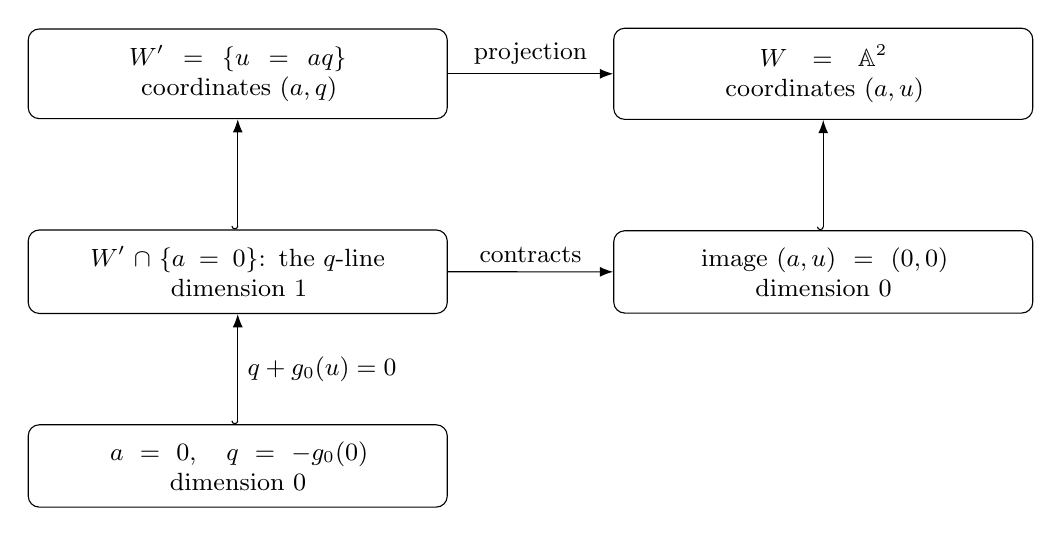
\begin{tikzpicture}[
  box/.style={draw,rounded corners,align=center,inner sep=6pt,
              text width=49mm,font=\small},
  >=Latex]
  \node[box] (graph) {$W'=\{u=aq\}$\\coordinates $(a,q)$};
  \node[box,right=21mm of graph] (base)
    {$W=\mathbb A^2$\\coordinates $(a,u)$};
  \node[box,below=14mm of graph] (fiber)
    {$W'\cap\{a=0\}$: the $q$-line\\dimension $1$};
  \node[box,below=14mm of base] (image)
    {image $(a,u)=(0,0)$\\dimension $0$};
  \draw[->] (graph) -- node[above,font=\small] {projection} (base);
  \draw[{Hooks[right]}->] (fiber) -- (graph);
  \draw[{Hooks[right]}->] (image) -- (base);
  \draw[->] (fiber) -- node[above,font=\small] {contracts} (image);
  \node[box,below=14mm of fiber] (point)
    {$a=0,\quad q=-g_0(0)$\\dimension $0$};
  \draw[{Hooks[right]}->] (point) --
    node[right,font=\small] {$q+g_0(u)=0$} (fiber);
\end{tikzpicture}

\caption{The graph $q=u/a$ over a two-dimensional affine base.
Horizontal arrows are projections and vertical arrows are inclusions.
The graph boundary is a line, but its image is a point.  The additional
equation $q+g_0(u)=0$ selects one point on that line, giving the
dimension $k-2=0$ used in the layer count.}
\label{fig:graph-projection}
\end{figure}

The next lemma gives a polynomial of low total degree with an arbitrarily
large prescribed polynomial ratio of order to degree.  Requiring
nonvanishing on the variety is part of the construction.

\begin{lemma}[Interpolation through successive layers]\label{lem:layer-interpolation}
Let $W'\subset\mathbb A^M$ be irreducible of dimension $k\geq1$,
with coordinates including $a,U,q$.  Let $\mathfrak b=(G_1,\ldots,G_t)$
have controlled generators and $V(\mathfrak b)=W'$.  Suppose
\[
 \dim V(\mathfrak b,a,F_0)\leq k-2,
 \qquad F_0=q+g_0(U),
\]
and put $F_n=F_0+\sum_{j=1}^{n-1}a^j g_j(U)$, where $m\ge1$ is an
integer and $\deg g_j\leq C(m+j+1)$.  Here $M,C$ are fixed and all other
complexities, including $m$, are polynomially bounded in $d$; the
coefficient heights through index $n$ are bounded by
$Q(n,d)\Psi(h)$.

For any prescribed positive integer $r$ polynomially bounded in $d$,
there are positive integers $L$ and $n=rL$, both polynomially bounded
in $d$, and a polynomial $P$ such that
\begin{equation}\label{eq:layer-membership}
 \deg P\leq L,\quad P\notin I(W'),\quad
 P=\sum_{\lambda=1}^t A_\lambda G_\lambda+A F_n+a^n B.
\end{equation}
The degrees of all the coefficients in this representation are
polynomial in $d$, and their joint affine height, including that of $P$,
is at most $Q'(d)\Psi(h)$.  The polynomial $Q'$ may depend on the
prescribed polynomial bound for $r$.
\end{lemma}

\begin{proof}
Fix a degree-compatible monomial order and a Gr\"obner basis of
$\mathfrak j=(\mathfrak b,a,F_0)$, together with representations of
its elements in these displayed generators.  Their degrees and heights
have the bounds recorded above.  For each reducible monomial, fix a
basis element to divide by.  Division in degree at most $T$ can then be
performed by a fixed decreasing sweep through all monomials of that
degree range, allowing zero coefficients.  Thus, for $\deg H\leq T$,
it gives linearly in $H$
\begin{equation}\label{eq:layer-division}
 H=\operatorname{rem}_{\mathfrak j}H
   +\sum_\lambda C_\lambda G_\lambda+aC+F_0D.
\end{equation}
There is a fixed bound $\Delta$, polynomial in the complexities at this
stage, such that every term on the right has degree at most $T+\Delta$.
Indeed, degree-compatible division produces quotient multipliers of
degree at most $T-\deg H_\alpha$ for a basis element $H_\alpha$.
Substituting its fixed generator representation adds its excess degree,
at most $\Delta$; it does not multiply $T$.

Work modulo $(\mathfrak b,F_n,a^n)$.  In
\eqref{eq:layer-division}, the $aC$ term advances one layer, while
\[
 F_0D\equiv-\sum_{j=1}^{n-1}a^jg_jD
\]
advances at least one layer.  Starting with a polynomial of degree at
most $L$, apply this division to each successive coefficient of
$1,a,\ldots,a^{n-1}$.  The coefficient being divided at layer $i$ has
degree at most $L+B_0(i+1)$, for a polynomially bounded $B_0$.
To verify this induction, a jump by $j\geq1$ adds at most
$\Delta+C(m+j+1)\leq B_0j$ to the degree.  The sum of all jumps to
layer $i$ is $i$, and there is no substitution at the same layer.
We retain every remainder and require it to be zero.

When $k=1$, the dimension hypothesis makes $\mathfrak j=(1)$, so there
are no remainder conditions.  If $\mathfrak j\ne(1)$, then $k\ge2$,
and the number of standard monomials of degree at most $T$ is at most
\[
 B_1(1+T)^{k-2},
\]
with $B_1$ polynomially bounded.  Here is an elementary uniform bound.
If the monomial initial ideal has generators of degree at most $D_1$,
in a standard monomial at most $\dim V(\mathfrak j)$ exponents can
be at least $D_1$.  Otherwise its variables of large exponent would
contain the support of a monomial generator, by the coordinate-prime
description of the radical of a monomial ideal.  Choose those variables
and bound every other exponent by $D_1-1$.  This gives the asserted
bound with a constant depending polynomially on $D_1$, since $M$ is
fixed.  If $\mathfrak j=(1)$ there are no standard monomials and no
conditions.  Thus at most
\begin{equation}\label{eq:layer-condition-count}
 B_1n(1+L+B_0n)^{k-2}
\end{equation}
linear conditions suffice when the ideal is proper.

Choose $k$ algebraically independent functions among the ambient
coordinate functions on $W'$.  Such a subset exists because these
functions generate its function field.  Let $V_L$ be the span of their
monomials of total degree at most $L$, regarded as actual polynomials
in the ambient coordinates.  Then
\[
 \dim V_L=\binom{L+k}{k},\qquad V_L\cap I(W')=0.
\]
This chooses independent polynomial representatives; no remainder map
is presumed to descend canonically to classes modulo $I(W')$.
One can equally extend $V_L$ to a linear complement of
$I(W')\cap\Qbar[a,U,q]_{\leq L}$.

Set $n=rL$.  For a proper $\mathfrak j$, the bound
\eqref{eq:layer-condition-count} is at most
\[
 B_2r(1+B_0r)^{k-2}L^{k-1}
\]
for a polynomially bounded $B_2$.  A sufficiently large polynomial
choice of $L$ makes it smaller than $\binom{L+k}{k}$.  In the unit-ideal
case the conclusion holds already for any nonzero source vector.
There is consequently a nonzero element $P\in V_L$ for which all
remainders vanish.  This proves both membership and $P\notin I(W')$.

For completeness, the construction also gives the asserted affine
height bounds.  Division in bounded degree is a linear operation on
a coefficient space of polynomial dimension.  During division the
leading monomial strictly decreases among the monomials of degree at
most $T$; thus its coefficient transformation is a product of
polynomially many matrices with controlled affine heights.  For
composable matrices with inner dimension $b$, the coefficient-tuple
convention gives
\[
 \ha{AB}\leq\ha{A}+\ha{B}+\log b.
\]
Indeed, locally every entry is a sum of $b$ products, and only infinite
places contribute the factor $b$.  The $n$ layer operations therefore have
polynomial affine heights.
Their source basis consists of monomials, so has height zero.  A kernel
vector obtained by minors and normalized to have a nonzero coordinate
equal to $1$ has affine height $Q(d,n,L)\Psi(h)$.

The tracked divisions give a membership representation of bounded
degree.  Alternatively, apply the arbitrary-membership bound to
$(\mathfrak b,F_n,a^n)$ and solve its coefficient equations with the
chosen $P$: the degrees and number of unknowns are polynomial in
$d,n,L$, and minors give the same affine height estimate.  This bounds
the scale of $P,A_\lambda,A,B$ together.  Since $r,L,n$ are polynomial
in $d$, \eqref{eq:layer-membership} follows with the stated bounds.
\end{proof}

\subsection{Product formula and descent}

\begin{proof}[Proof of \Cref{thm:interpolation}]
We descend through irreducible subvarieties $W\subseteq X$ containing
$z_*$.  At every step their degrees and degrees of chosen
set-theoretic equations are polynomial in $d$, and the affine heights
of those equations are at most $Q(d)\Psi(h)$.  Initially take a
component of $X$ containing the point.  The algebraic bounds above
preserve these conditions under each operation below.

If $a$ is constant on $W$, its constant value has height at most
$Q(d)\Psi(h)$, by projection to the $a$-line and the component height
bound.  On the other hand the product formula and
\eqref{eq:interpolation-smallness} give
\begin{equation}\label{eq:constant-parameter-height}
 \ha{a_*}=\sum_vw_v\log\max(1,\abs{a_*}_v^{-1})
 \geq S_{\rm small}\geq h/Q_1(d).
\end{equation}
Hence $h\leq Q(d)\Psi(h)$, which implies a polynomial bound in $d$:
for fixed $c$, $1+(\log h)^c\leq C_c\sqrt h$ for $h\geq2$.

Suppose now that $a$ is nonconstant and $k=\dim W\geq1$.
If $a$ is nonconstant but $V_W(a)$ is empty, this case can be settled
without an analytic equation.  For the controlled ideal
$\mathfrak b_W=(G_1,\ldots,G_t)$, the ideal $(\mathfrak b_W,a)$ is the
unit ideal.  The membership and coefficient bounds provide
\[
 1=\sum_i A_iG_i+aB
\]
with polynomial degrees in $d$ and joint affine height
$Q(d)\Psi(h)$.  At the target $1=a_*B(z_*)$.  Evaluating $B$ on the
selected embeddings costs only its coefficient height and the small
local sizes of $U_*$, since $\abs{a_*}_v<1$.  It follows that
\[
 S_{\rm small}=\sum_{v\in\mathcal V}w_v\log\abs{B(z_*)}_v
 \leq Q(d)\Psi(h).
\]
Again $h\leq Q(d)\Psi(h)$ gives the required polynomial bound.
We may therefore suppose that $V_W(a)$ is nonempty.

The total number of generic normalization branches above $V_W(a)$ is
at most $\deg W$.  Indeed take one general transverse linear slice
meeting every component $D_j$ of this fibre at general affine points.
The curve components have total degree at most $\deg W$.  Their
normalizations contain the transverse germs above all these points.
If a normalization divisor above $D_j$ has residue degree $f_i$ and
$e_i=\operatorname{ord}_i(a)$, it contributes
$\deg(D_j)f_ie_i$ to the zero divisor of $a$ on the normalized slice.
That divisor has degree equal to the polar degree of $a$, at most
$\deg W$.  In particular the number of branches is bounded.  This
counts residue degrees and ramification multiplicities, even though
the normalization itself is birational.

At each such branch choose the lowest nonzero order among the $E_\nu$.
To avoid cancellation of these leading terms in a combination, set
\[
 E=\sum_{\nu=1}^s t^{\nu-1}E_\nu
\]
for a positive integer $t$.  Each branch excludes at most $s-1$ values
of $t$, since its leading-coefficient polynomial is nonzero.  There is
therefore a permissible $t$ of polynomial size in $d$.  This combination preserves
the coefficient and tail bounds: at finite places its coefficients
are integral, and the extra triangle-inequality factor at infinite
places has total logarithm polynomial in $d$.  Absorb it in the $b_v$.
Write $E=\sum a^j e_j(U)$.

By \Cref{lem:zero-estimate}, an integer $m$ polynomially bounded in
$d$ can be chosen so that, for
\[
 f=\sum_{j=0}^{m-1}a^je_j(U),
\]
one has $\operatorname{ord}_{\mathfrak p}f
<m\operatorname{ord}_{\mathfrak p}a$ on every relevant branch.
Indeed the omitted terms have order at least
$m\operatorname{ord}_{\mathfrak p}a$, since all their coefficients
are regular on the affine variety.  Form the graph $W'$ of
$q=f/a^m$.  Its equations with controlled support are obtained by
saturating $(\mathfrak b_W,a^mq-f)$ by $a$; the closure of its support
is exactly the graph.  This takes place in one more variable and
has polynomial degree and affine height bounds.

The target lifts to $z_*'=(a_*,U_*,q_*)$.  Its global height is bounded
using the rational expression for $q_*$:
\begin{equation}\label{eq:graph-global-height}
 \ha{z_*'}\leq Q_5(d)h+Q_6(d)\Psi(h).
\end{equation}
Here $Q_5$ is fixed at this stage, before the interpolation degree and
order are chosen.  Its selected local size must instead be estimated
using the exact equation $E(z_*)=0$.  The tail bound gives
\begin{equation}\label{eq:graph-local-height}
 \abs{q_*}_v
 =\left|a_*^{-m}\sum_{j\geq m}a_*^je_j(U_*)\right|_v
 \leq\exp((m+1)b_v).
\end{equation}
In particular the sum of the positive local logarithmic sizes of
$(U_*,q_*)$ is at most $Q_7(d)\Psi(h)$.
The new equation and its finite truncations are
\[
 F=q+\sum_{j\geq0}a^je_{m+j}(U),\qquad
 F_n=q+\sum_{j=0}^{n-1}a^je_{m+j}(U).
\]
At the target,
\begin{equation}\label{eq:shifted-tail}
 \abs{F_n(z_*')}_v
 \leq\abs{a_*}_v^n\exp((m+n+1)b_v).
\end{equation}

By \Cref{lem:graph-fiber},
$V(I(W'),a,q+e_m)$ has dimension at most $k-2$.
For a controlled ideal $\mathfrak b$ defining $W'$ set-theoretically,
$V(\mathfrak b,a,q+e_m)$ is the same set and has the same dimension.
Apply \Cref{lem:layer-interpolation}, with the ratio $r=n/L$ to be
chosen shortly.  At the lifted target its identity becomes
\[
 P(z_*')=A(z_*')F_n(z_*')+a_*^nB(z_*').
\]
Equations \eqref{eq:polynomial-evaluation},
\eqref{eq:graph-local-height}, and \eqref{eq:shifted-tail}, together
with the coefficient and membership degree bounds, imply
\begin{equation}\label{eq:local-interpolation-value}
 \sum_{v\in\mathcal V}w_v\log\abs{P(z_*')}_v
 \leq -n S_{\rm small}+Q_8(d,n,L)\Psi(h).
\end{equation}
All positive contributions here are sums of affine coefficient heights,
positive local coordinate sizes, the $b_v$, and infinite-place
triangle-inequality terms.  There is no error proportional to the
number of finite places.
At the remaining places evaluate $P$ itself, rather than its membership
representation.  Since $\deg P\leq L$, \eqref{eq:graph-global-height}
gives
\begin{equation}\label{eq:outside-interpolation-value}
 \sum_{v\notin\mathcal V}w_v\log\abs{P(z_*')}_v
 \leq LQ_5(d)h+Q_9(d,n,L)\Psi(h).
\end{equation}

The choices can now be made in the required order.  The graph and
$m$ have already fixed $Q_5$.  Choose an integer
$r>2Q_1(d)(Q_5(d)+1)+1$, polynomially bounded in $d$.
Next choose the polynomially large $L$ supplied by
\Cref{lem:layer-interpolation}, and set $n=rL$.
If $P(z_*')\ne0$, its product formula and
\eqref{eq:local-interpolation-value}--\eqref{eq:outside-interpolation-value}
give
\[
 0\leq
 \left(-\frac n{Q_1(d)}+LQ_5(d)\right)h
 +Q_{10}(d,n,L)\Psi(h).
\]
The coefficient of $h$ is at most $-L$.  As $n,L$ are now fixed
polynomials in $d$, this inequality
again implies $h\leq Q(d)\Psi(h)$ and hence a polynomial height
bound.  Thus, beyond a polynomial threshold chosen \emph{after}
$m,r,L,n$, the value $P(z_*')$ must be zero.

Since $P\notin I(W')$, the intersection $W'\cap V(P)$ has dimension
at most $k-1$.  Project it to the original $(a,U)$-space, take its
closure, and choose an irreducible component containing $z_*$.  Such
a component exists because $a_*\ne0$ and the graph projection is an
isomorphism over that open set.  Projection cannot increase dimension.
The degree and arithmetic bounds above preserve the induction
hypotheses.  Discard the graph coordinate $q$; at the next step construct
a new graph from the original common equations on this smaller
variety.  Consequently the ambient number of variables stays fixed.

The dimension drops at every continuing step, so there are at most
$\dim X$ such steps.  A zero-dimensional final variety has constant
$a$ and is covered by \eqref{eq:constant-parameter-height}.  Taking the
maximum of the finitely many polynomial thresholds proves the theorem.
All component and coefficient field extensions made during the proof
extend the selected local data by all embeddings, as specified above;
they do not alter any smallness sum or introduce a field-degree factor.
\end{proof}

\section{Arithmetic coordinates and common local relations}\label{sec:arithmetic}

We construct the algebraic coordinates and common local equations needed
for \Cref{thm:interpolation}.  The coordinates will have controlled global
height and much smaller norms on the center disks.  A weighted proximity
estimate then ensures that one common system of equations retains enough
smallness of the local parameter.  Throughout this section the curve, its
finite cover, its algebraic frames, and the center are fixed.  In
particular the conclusions apply after any one fixed auxiliary level
cover.  No condition on the reduction type of the center is imposed.

Write $\pi:\mathcal A\to S$ for the abelian scheme and put
$\mathcal H=R^1\pi_*\Omega^\bullet_{\mathcal A/S}$.  We use the
operator realization of $\Vcal\subset\End(\mathcal H)$ from
\Cref{lem:qm-plane}.  On actual endomorphisms, $\Tr$ denotes the trace
on first cohomology, so that $\Tr(1)=4$.  As in
\eqref{eq:quadratic-system}, $\pair{u}{v}=\tfrac14\Tr(uv)$.
For an endomorphism $u$, set
\[
 q_\lambda(u)=\Tr(uu^\dagger),
\]
where $\dagger$ is the principal Rosati involution.  This is a positive
definite integral quadratic form on $\End(A)$.

For a number field $F$ containing coordinates under consideration, our
weights are $w_v=[F_v:\Q_v]/[F:\Q]$, with the usual unsquared absolute
values.  Thus $\ha{z}=\sum_v w_v\log\max(1,\norm{z}_v)$ for an
affine tuple $z$, where the norm is the coordinate maximum.  The same sums
can be written over embeddings into $\C$ or $\overline{\Q}_p$, giving
each embedding weight $1/[F:\Q]$.  If a selected set of embeddings is
extended to a larger field, we always take \emph{all} extensions.  Their
weights sum to the old weight.  This convention also permits grouping
embeddings in a normal closure without charging its degree to any estimate.

After omitting finitely many points, fix a rational frame of $\Vcal$
regular at $t_0$, affine coordinates $z$ on a neighborhood of $t_0$, and
$x\in K(S)$ with a simple zero at $t_0$.  The inverse branch through
$t_0$ is denoted $z=z(X)$, with $z(0)=z(t_0)$.  Shrink the neighborhood
so that these data and the connection are regular there.
Choose two independent integral trace-free Rosati-symmetric endomorphisms
of $A_{t_0}$ as in \Cref{lem:qm-plane}, enlarge $K$ once to define them,
and denote their de Rham coordinate pair by $B=(B_1,B_2)$.
For ordered vector pairs $\mathbf v=(v_1,v_2)$ and
$\mathbf w=(w_1,w_2)$, write
$\pair{\mathbf v}{\mathbf w}=(\pair{v_i}{w_j})_{i,j=1}^2$.
Put
$a=x(t)\ne0$, $h=\max\{2,h_H(t)\}$ for a fixed nonnegative
ample logarithmic height on $\overline S$, and
$d=\max\{2,[K(t):K]\}$.
All constants below depend only on the fixed data.

\subsection{Integral endomorphisms and de Rham coordinates}

\begin{lemma}[Potential good reduction]\label{lem:potential-good}
An abelian surface whose geometric endomorphism algebra is a quaternion
division algebra over $\Q$ has potentially good reduction at every finite
place.
\end{lemma}

\begin{proof}
Fix a finite place.  The semistable reduction theorem
\cite[Section~7.4, Theorem~1]{BLR1990}, followed by a further finite
extension, gives semistable reduction and defines all geometric
endomorphisms.  They extend to the N\'eron model and preserve
the torus in its connected special fiber.  If that torus has positive
rank $r$, its rational character space is a nonzero unital module, on
one side or the other, for the division algebra
$D=\End^0(A_{\overline K})$.  Every finite dimensional module over a
division algebra is free over it, so its rational dimension is a
positive multiple of $\dim_\Q D=4$.  This contradicts $r\le2$.
The toric rank is therefore zero, and the semistable model is an
abelian scheme.  The extension used here is local; no uniform bound on
its degree is needed for an absolute height computation.
\end{proof}

\begin{proposition}[Small labeled integral vectors]\label{prop:small-vectors}
There are constants $c,C>0$ with the following property.  For every
target $t$, an extension $L/K(t)$ of degree at most $C$ defines all
geometric endomorphisms of $A_t$.  There are two independent
endomorphisms $u_1,u_2\in\End_L(A_t)$ which are symmetric and trace
free, span $E_t$, and satisfy
\begin{equation}\label{eq:rosati-size}
 q_{\lambda_t}(u_j)\le C(dh)^c\qquad(j=1,2).
\end{equation}
The corresponding labeled vectors are denoted $P=(P_1,P_2)$ in de Rham
coordinates.  Conjugating a labeled target always means conjugating
these endomorphisms as well.  This pair need not generate the saturated
integral cohomology lattice of $E_t$.
\end{proposition}

\begin{proof}
The Galois action on the geometric endomorphism lattice has finite
image in $\mathrm{GL}_r(\Z)$, with $r\le16$.  Indeed a finite set of
lattice generators is defined over a finite extension.  A finite
subgroup of $\mathrm{GL}_r(\Z)$ injects into
$\mathrm{GL}_r(\mathbf F_3)$, because the kernel of reduction modulo
$3$ is torsion free.  Its order is consequently bounded in terms of
$r$ alone.  The fixed field of the kernel gives the asserted $L$.

For a principally polarized abelian variety of fixed dimension, the
endomorphism estimate of Masser--W\"ustholz gives a rational spanning
set of integral endomorphisms whose Rosati lengths are bounded by a
fixed power of
\[
 \max\{2,[L:\Q],h_F(A_t)\}.
\]
Here polynomial dependence on the field degree is essential.  It is
explicit in the Proposition of \cite[Section~4]{MW1994}, with its
parameter $m$ equal to the dimension of the abelian variety; the
alternative involving a smaller image is then zero.  Its lattice
Lemma~2.1 also gives a basis with the same kind of bound.  See also
\cite[Theorem~6.6 and Section~6.7]{DawOrr2022} for the polynomial
dependence in this application.  The theta-height comparison
\cite[Theorem~1.1 and Corollary~1.3]{Pazuki2012}, on one fixed theta
level, and functoriality of heights on a fixed curve give
\[
 h_F(A_t)\le C h.
\]
The degree of passage to that fixed level is bounded.

For clarity, the projection to the required plane can be made without
target-dependent denominators.  The map
\[
 u\longmapsto 4(u+u^\dagger)-\Tr(u+u^\dagger)1
\]
preserves integrality, has symmetric trace-free image, and increases
the Rosati norm by at most a fixed factor.  By
\Cref{lem:qm-plane} its rational image has dimension two.  Apply this
map to the small spanning set and select two independent images.
This proves \eqref{eq:rosati-size}.  The norm and trace assertions are
unchanged under field conjugacy: they are traces of actual
endomorphisms and their Rosati adjoints.
\end{proof}

The next distinction is useful.  A rational frame can have large
denominators at a moving point, even when the endomorphism is integral.
Their global cost is linear in $h$.  On fixed sufficiently small
neighborhoods of the center the frames are uniformly controlled, and
the restricted cost is much smaller.

\begin{proposition}[Coordinate heights and local norms]\label{prop:dr-size}
Choose the vectors of \Cref{prop:small-vectors}.  Their affine
coordinates in the fixed frame satisfy
\begin{equation}\label{eq:dr-global}
 \ha{z(t),a,P}\le C(h+\log d).
\end{equation}
There are center neighborhoods at every place, with a single integral
description outside a fixed finite set of rational primes, such that
for any selected weighted set $\mathcal V$ on the actual center branches,
\begin{equation}\label{eq:dr-local}
 \sum_{v\in\mathcal V}w_v
       \log\max(1,\norm{z(t),P}_v)
       \le C(1+\log h+\log d).
\end{equation}
These statements hold for the finitely many conjugate fixed charts.
They also hold after a bounded denominator and a polarized isogeny
of any one fixed multiplier are applied to the vectors.
\end{proposition}

\begin{proof}
\emph{Global finite-place bounds.}
We first bound the denominators of integral endomorphisms in the rational
frame.  Potential good reduction supplies an integral de Rham lattice at
each target; a fixed ideal measures the denominators of the frame and
its dual relative to that lattice.  Pass,
for this argument only, to a fixed common cover carrying two coprime
fine levels $N_1,N_2\ge3$.  The integral fine moduli scheme
$\Acal_2(N_i)$ is quasi-projective over $\Ocal_K[1/N_i]$
\cite[Chapter~I, Theorem~1.4 and Section~1.7]{Chai1985}.
Embed it in projective space over this ring, take its scheme-theoretic
closure, and then take the closure of the graph of the curve map in
the product with the fixed projective curve model.
Denote this proper graph
model by $X_i$.  Take its projective closure over $\Ocal_K$ when
using global model heights.  The inverse image $U_i$ of the abelian interior
carries the integral vector bundle $\mathcal H_i$ of first de Rham
cohomology and its dual.  At a prime $p\nmid N_i$, a target acquires
good reduction by \Cref{lem:potential-good}; its prime-to-$p$ level
extends after a finite local extension.  Properness extends the
point to $X_i$.  The good-reduction abelian scheme with prime-to-$p$
level also supplies a valuation-ring point of the abelian interior.
Its map to the projective closure agrees with the graph map on the
generic fiber, hence everywhere by separatedness.  The moduli image
of the extended graph point therefore lies in the abelian interior.
Consequently the extended point belongs to $U_i$.

This last assertion concerns the moduli image.  The point is allowed
to reduce above a boundary point of the original curve.  Thus we use
$U_i$, rather than a preassigned integral open of the curve, to
compare lattices.  The two choices of $i$ cover every residue
characteristic.

Choose a rational frame $e_1,\ldots,e_4$ of $\mathcal H$ such that it
and its dual $e^1,\ldots,e^4$ are regular at $t_0$.  Form on $U_i$ the
coherent denominator ideals
\[
 \mathcal I_+=\{f:f e_j\in\mathcal H_i\text{ for all }j\},
 \qquad
 \mathcal I_-=\{f:f e^j\in\mathcal H_i^\vee\text{ for all }j\}.
\]
These are coherent colon ideals, and extend to coherent ideals on
the noetherian projective model $X_i$
\cite[Lemma~28.23.1(2), Tag~01PE]{StacksProject}.  Their product, further
multiplied by a denominator ideal for the fixed rational conversion
from operator entries to our frame of $\Vcal$, gives a fixed ideal
$\mathcal J_i$.  Multiplication by $\mathcal J_i$ makes all the
specified sections integral on $U_i$.  Remove its finitely many
generic zeros from the curve.  No duality assertion about arbitrary
coherent extensions across the boundary is required.
For a lifted target over a valuation ring $R$, write
$\mathcal J_i(t)R=(\eta)$ and
$\Lambda=H^1_{\mathrm{dR}}(\mathcal A_t/R)$.  The frame vectors
belong to $\eta^{-1}\Lambda$ and their duals belong to
$\eta^{-1}\Lambda^\vee$.  An actual integral endomorphism preserves
$\Lambda$: it extends to the abelian scheme
\cite[Section~1.2, Proposition~8]{BLR1990}, and de Rham cohomology
is functorial.  Each of its matrix entries is therefore in
$\eta^{-2}R$.  The extra fixed conversion of coordinates gives,
for some fixed integer $b$,
\begin{equation}\label{eq:pole-ideal}
 \log\max(1,\norm{P}_v)
       \le b\lambda_{\mathcal J_i,v}(t)+c_v
       \quad(v\nmid N_i),
\end{equation}
where $c_v=0$ outside finitely many fixed primes.

Here is explicitly why the right side has the claimed global cost.
For a sufficiently ample fixed line bundle $\mathcal L$ on $X_i$,
$\mathcal J_i\mathcal L^n$ is generated by finitely many fixed
sections $s_0,\ldots,s_r$
\cite[Proposition~28.27.13(7), Tag~01Q3]{StacksProject}.
Choose $s_k$ with $s_k(t)\ne0$.
With the model norm at a finite place,
$\lambda_{\mathcal J_i,v}(t)\le-\log\norm{s_k(t)}_v$.
The product formula for this nonzero element of the metrized line
$\mathcal L_t^n$ gives
\[
 \sum_{v\nmid\infty}w_v\lambda_{\mathcal J_i,v}(t)
 \le n h_{\mathcal L}(t)
       +\sum_{v\mid\infty}w_v\log\norm{s_k(t)}_v
 \le n h_{\mathcal L}(t)+C.
\]
The last bound uses the bounded sup norms of the finitely many
fixed sections on the fixed projective complex model.  The finite
ideal heights are nonnegative, so this also bounds any restricted
finite sum, such as the sum over $p\nmid N_i$.
Every generic projective curve and map used here is fixed, so
$h_{\mathcal L}(t)=O(h)$.  Equation \eqref{eq:pole-ideal}, summed
using the two models, bounds all finite denominator contributions
by $O(h)$, independently of the local extension used for good
reduction.

\emph{Global archimedean bounds.}
At an archimedean place the Hodge norm of an actual endomorphism is
$q_{\lambda_t}^{1/2}$, up to a fixed convention.  In a rational de
Rham frame, the norms of the frame and dual have at most a fixed
power of the inverse distance to the finitely many omitted points,
times powers of its logarithm.  The algebraic Gauss--Manin connection
is regular singular by \cite[Theorem~14.1]{Katz1970}; this property
passes to its duals, tensor products and subquotients
\cite[Proposition~11.3 and Remark~11.3.4]{Katz1970}.
After a fixed ramified cover at each puncture, compare its algebraic
logarithmic lattice with the canonical extension of the variation.
Both frames and their inverses differ by meromorphic matrices with
finite pole orders.  Schmid's norm estimates for the variation and
its dual \cite[Theorems~4.9 and~6.6$'$]{Schmid1973} then give the
asserted power and logarithmic bounds for the rational frame and its
dual.  The sum of the positive logarithms of these factors is
$O(h)$ by the local height inequalities for the fixed omitted
divisor.  The contribution of \eqref{eq:rosati-size} is
$O(\log h+\log d)$.  Affine base coordinates and $a$ are fixed
rational functions and have height $O(h)$.  This proves
\eqref{eq:dr-global}.

\emph{Bounds on the center disks.}
For \eqref{eq:dr-local}, outside finitely many primes the family,
parameter chart, frame, and dual are integral near the center,
with the frame invertible.  All integral endomorphism coordinates
then have norm at most one on that residue neighborhood.  At a fixed exceptional prime $p$, extend the local coefficient
field once so that the fixed center has good reduction and a
chosen full $M$-level structure, where $M\ge3$ and $p\nmid M$.
Adding this level to the original characteristic-zero curve
gives a finite \'etale cover; at the chosen lift of the center,
the $p$-adic inverse function theorem gives an analytic section
over a sufficiently small center disk.  Every sufficiently
close target on the original branch therefore has a lift on
this section after coefficient extension, including when the
original level is divisible by $p$.  Forgetting the original
level maps the lifted disk to the prime-to-$p$ fine moduli
scheme.  On a smaller closed disk its coordinates lie in an
integral open about the fixed center and reduce to the same
special point.  An integral de Rham frame on this moduli open
pulls back to a frame whose change-of-basis matrix with the
original frame, and its inverse, are analytic and bounded on
the disk.  Thus both the finite-place comparison cost and the
base-coordinate norms are bounded by fixed local constants.

At infinity choose compact
disks within the regular charts; the frame and dual Hodge norms
are bounded there.  Only $O(\log h+\log d)$ remains from the
Rosati norm.  The sum of weights above a fixed rational prime is
one, as is the sum of archimedean weights, which proves the
restricted sum.

Finally a polarized isogeny of fixed multiplier carries Rosati
norms isometrically under conjugation on operators.  Its inverse
introduces only a bounded denominator into an actual
endomorphism.  This changes the finite estimates at finitely many
fixed primes by fixed constants, and proves the last assertion.
\end{proof}

\subsection{Horizontal comparison on good-reduction disks}

We next express pairings between centered and target endomorphisms in
one cohomology space.  At finite places the common special fiber supplies
that space, and functorial comparison must apply to each individual
endomorphism even when it does not extend over the base curve.
Let $Y(X)$ be the rank-five horizontal transport \emph{back} to the
center, normalized by $Y(0)=I$.  It is obtained from the corresponding
transport on $\mathcal H$ by the operator construction.  Its entries
are ordinary-point Taylor series over $K$.

\begin{proposition}[Functorial good-reduction comparison]\label{prop:good-comparison}
At a finite place, suppose a point $t$ is on a sufficiently small
actual center branch.  After coefficient extension the two
polarized abelian schemes have a common special fiber $\overline A$.
More precisely, over a finite local extension $F$ with residue
field $k$, put $F_0=W(k)[1/p]$ and
$D=H^1_{\mathrm{cris}}(\overline A/W(k))[1/p]$.  There are rational
comparison isomorphisms
\[
 c_u:H^1_{\mathrm{dR}}(A_u/F)\longrightarrow D\otimes_{F_0}F,
 \qquad u=t_0,t,
\]
whose transition $c_{t_0}^{-1}c_t$ is horizontal transport.
They are compatible with morphisms of either lifted fiber and
their specializations, including morphisms which do not extend
over the base curve.  Ramification of the coefficient field is
allowed.

In particular, if $\beta_i$ and $\alpha_j$ are the specializations
of the centered and target endomorphisms, then
\begin{equation}\label{eq:cross-trace}
 \pair{B_i}{Y(a)P_j}=\tfrac14\Tr(\beta_i\alpha_j)\in\Q
       \qquad(1\le i,j\le2).
\end{equation}
The cross pairings belong to $\tfrac14\Z$, and their ordinary
absolute values are at most $C(dh)^c$.  At archimedean places the
same assertions hold with integral Betti transport in place of
specialization.
\end{proposition}

\begin{proof}
Work on a smooth integral prime-to-$p$ fine moduli chart
$\mathfrak M$ over a Witt base, and let $z$ be the common
special point.  The relative first crystalline cohomology of
the universal abelian scheme defines a convergent isocrystal
$\mathcal E$ on the special fiber of this chart.  Its value
at $z$ is the crystalline cohomology of the actual abelian
variety $\overline A$ over $z$.  The canonical realization of
$\mathcal E$ on any smooth proper lifting is its relative
de Rham cohomology with Gauss--Manin connection; see
\cite[Theorems~4.16 and~4.26]{MaulikPoonen2012}, the latter
using \cite[Theorem~3.8.2]{Ogus1984}.

Here is the common evaluation explicitly.  Over the local
field $F$ in the statement, put
$\mathfrak T=\operatorname{Spf}\Ocal_F\langle Z\rangle$
and substitute $X=aZ$ into the chosen inverse branch.  Shrinking the
fixed center disks ensures that the resulting chart coordinates belong
to $\Ocal_F\langle Z\rangle$ and differ from their centered values by
elements of $\mathfrak m_F\Ocal_F\langle Z\rangle$, where
$\mathfrak m_F$ is the maximal ideal of $\Ocal_F$.  Thus the map to
$\mathfrak M$ reduces constantly to $z$ on
$(\mathfrak T\bmod p)_{\mathrm{red}}=\operatorname{Spec}k[Z]$.
This remains true when $F$ is ramified and $a\notin p\Ocal_F$:
the image of $\mathfrak m_F$ in $\Ocal_F/p$ is nilpotent.
Consequently $\mathfrak T$ is an enlargement of $z$, and
the crystal transition for its structural map to the point
enlargement gives a canonical horizontal identification
\[
 \mathcal E_{\mathfrak T}
   \simeq D\otimes_{F_0}\Ocal_{\mathfrak T}[1/p].
\]
This is the constant-reduction construction of
\cite[Definitions~4.10--4.13 and Section~4.7]{MaulikPoonen2012}.

At $Z=0$ and $Z=1$, the relative comparison gives precisely
the two maps $c_{t_0}$ and $c_t$ of the statement.  Their
compatibility with restriction to a fiber identifies them
with the functorial absolute crystalline--de Rham
comparisons; an explicit absolute statement with arbitrary
ramification is
\cite[Appendix~B, Proposition~B.4]{KubrakPrikhodko2022}.
Proper formal GAGA identifies completed and ordinary
de Rham cohomology.  An endomorphism of either individual
fiber extends over its good-reduction abelian scheme and
is carried to its actual specialization on $\overline A$.
This argument needs only that individual endomorphism,
without an extension to neighboring fibers.  The common
fiber is $\overline A$ itself, with the same specialization
maps and prime-to-$p$ markings as in smooth proper base
change.  The construction does not introduce an auxiliary
isogeny between special fibers.

The crystal identification is horizontal and is the
identity when the two evaluations coincide.  Therefore
$c_{t_0}^{-1}c_t$ is the identity-normalized horizontal
transport, and uniqueness for the ordinary differential
equation identifies its operator realization with $Y(a)$.
The resulting relative matrix identity is also discussed
in \cite[Theorem~3.4 and Remark~3.6]{PapasI2025}.

Outside finitely many
fixed primes our curve chart and connection are integral; the
Taylor comparison converges, including over ramified extensions,
whenever
\begin{equation}\label{eq:factorial-disk}
 -\log|a|_v>\frac{2\log p}{p-1}.
\end{equation}
Indeed the divided-power terms have denominators dividing the
corresponding factorial.  At the finitely many other primes,
\Cref{lem:potential-good} for the fixed center and a
prime-to-characteristic moduli chart give the same assertion on
a fixed smaller disk.

Functoriality identifies both operator realizations with the
operators $\beta_i,\alpha_j$ on the same crystalline vector
space, proving \eqref{eq:cross-trace}.  The characteristic
polynomial of an endomorphism of an abelian variety has integral
coefficients and is independent of the Weil cohomology: it is
characterized by the degree polynomial $\deg(n-u)$
\cite[Section~12]{Milne1986}.  For the crystalline realization used
here, the cohomological assertion can be seen directly.  Rational
crystalline cohomology is a Weil cohomology
\cite[Remark~4.15]{MaulikPoonen2012}.  Cup product identifies the
cohomology of the abelian special fiber with the exterior algebra on
$H^1$: comparison with its good lift reduces this to the corresponding
statement for a complex abelian variety.  Thus $[n]-u$ acts on top
cohomology by $\det(n-u\mid H^1)$; the degree formula identifies that
action with $\deg([n]-u)$.  Equality for all sufficiently large integers
$n$ identifies the characteristic polynomials, and hence their traces.
This applies
also to $\beta_i\alpha_j$, so its trace is integral and the pairing
in \eqref{eq:cross-trace} belongs to $\tfrac14\Z$.  Specialization
preserves the polarization, Rosati involution, and these trace
polynomials.  Positivity of the Rosati form in characteristic
$p$ \cite[Theorem~17.3]{Milne1986} gives
\[
 |\Tr(\beta_i\alpha_j)|^2
 \le \Tr(\beta_i^2)\Tr(\alpha_j^2)
 \le C(dh)^c.
\]
At infinity parallel transport identifies integral first
cohomology lattices, so the cross pairing again belongs to
$\tfrac14\Z$.  On
the compact center disk the Hodge norms at the two points are
uniformly comparable under this transport.  Cauchy--Schwarz for
the resulting positive norm and \eqref{eq:rosati-size} give the
same size bound.  Notice that the two transported operators need
not both be Hodge endomorphisms at the center in this last argument.
\end{proof}

\subsection{Smallness on the actual center branches}

\begin{lemma}[Proximity and the factorial cutoff]\label{lem:proximity}
Use the fixed center disks of \Cref{prop:dr-size,prop:good-comparison},
and at every remaining prime impose \eqref{eq:factorial-disk}.
Let $\mathcal V_0(t)$ be all weighted embeddings at which $t$
belongs to these actual branches.  Then
\begin{equation}\label{eq:proximity-sum}
 \sum_{v\in\mathcal V_0(t)}w_v\log(1/|a|_v)
       \ge c h-C\bigl(1+\log^2(dh)\bigr).
\end{equation}
In particular the sum is at least $c h/2$ if $h\ge Q_0(d)$
for a fixed polynomial $Q_0$.
\end{lemma}

\begin{proof}
Use the effective divisor $D_0=[t_0]$ on the smooth completion
$\overline S$.  Since it has positive degree, some fixed multiple
of $D_0$ minus the ample divisor defining $h$ is ample.  The
height of an ample divisor is bounded below, and hence
\[
 h_{D_0}(t)\ge c h-C.
\]
Take local Weil functions for this divisor.  On the actual
branch through $t_0$ they equal $-\log|x(t)|_v$ up to fixed
bounded errors.  Outside the chosen branch neighborhoods their
positive contributions are bounded; the error is zero at all
but finitely many primes.  At an unexceptional prime the
integral parameter chart is \'etale at the center, so the branch
is precisely the Henselian inverse branch with that reduction.
Other zeros of the rational function $x$ are not counted.
Before the factorial cutoff, the weighted proximity sum is
therefore at least $ch-C$.

Here is a uniform bound for the loss caused by that cutoff.  Put
$D=[K(a):\Q]\le Cd$ and $H=\ha{a}\le Ch$.  If a rational prime
$p$ has any place where $|a|_v<1$, it contributes at least
$(\log p)/D$ to $\ha{a^{-1}}=H$: writing a local valuation in
integral units cancels its ramification index against the
absolute weight.  For the set $\mathcal P(a)$ of these primes,
\begin{equation}\label{eq:prime-support}
 \sum_{p\in\mathcal P(a)}\log p\le DH,
 \qquad \#\mathcal P(a)\le DH/\log2.
\end{equation}
Write $\alpha_p=\log p/(p-1)$.  At places over $p$ discarded
by \eqref{eq:factorial-disk}, the total weighted loss is at
most $2\alpha_p$, since their weights sum to at most one.
For any set of $N$ primes,
\[
 \sum\alpha_p
 \le C\sum_{k=1}^{N}\frac{\log(k+1)}k
 \le C\bigl(1+\log^2(N+1)\bigr).
\]
Here $\log x/(x-1)$ decreases for $x>1$, and the $k$th
smallest prime is at least $k+1$.  Apply this with
\eqref{eq:prime-support}.  Restricting the finitely many
exceptional and archimedean disks costs only a fixed further
constant.  This proves \eqref{eq:proximity-sum}; its last
assertion follows by elementary absorption of the logarithmic
term for $h\ge Q_0(d)$.
\end{proof}

\subsection{Grouping the equations}

Include in the fixed exceptional set all denominator primes of the
centered vectors and the trace pairing, in all fixed conjugate charts.
At infinity and at the finitely many exceptional primes, only $O(d)$
embeddings of the labeled field occur, so we can keep the rational
cross-trace matrix as a coefficient of each group's equations.  The
number of remaining primes can grow with the target.  There we compare
a trace equation with its image under a lift of residue Frobenius.
The rational trace is fixed, so subtraction eliminates it; only $O(d)$
conjugates of the complete labeled tuple can occur.  Retaining the labels
also records Frobenius's action on the actual endomorphisms, as needed
in \Cref{sec:height}.

\begin{proposition}[Common relations with controlled coefficients]
\label{prop:common-relations}
Suppose $h\ge Q_0(d)$, increasing $Q_0$ if necessary.  The
proximity embeddings can be partitioned into at most $Q_1(d)$
groups, and one group $\mathcal V$ has
\begin{equation}\label{eq:group-smallness}
 S_{\mathrm{small}}=
 \sum_{v\in\mathcal V}w_v\log(1/|a|_v)
       \ge h/Q_2(d).
\end{equation}
On each group there is one fixed list of analytic equations,
evaluated at one algebraic tuple $(a,U)$, of one of the following
forms:
\begin{align}
 \pair{B}{Y(a)P}&=T,
       &&\text{with }T\in\mathrm{M}_2(\Q),
       \label{eq:constant-relations}\\
 \pair{B}{Y(a)P}&=\pair{B'}{Y'(aR)P'},
       &&R=b/a,\quad b=x'(t'),
       \label{eq:paired-relations}
\end{align}
together with the actual branch equations
\begin{equation}\label{eq:chart-relations}
 z-z(a)=0,
 \qquad z'-z'(aR)=0
 \quad\text{when a second chart is present}.
\end{equation}
The primed data are one simultaneous field conjugate of the
complete labeled unprimed data.  In \eqref{eq:paired-relations}
all places are finite and $|R|_v=1$ on the group.  The Frobenius
of the common reduction transports each of the two labeled
pairs to its primed pair.

The tuple has degree at most $Q_3(d)$ over $K$, and
\begin{equation}\label{eq:common-size}
 \ha{a,U}\le Q_3(d)h,
 \qquad
 \sum_{v\in\mathcal V}w_v\log\max(1,\norm{U}_v)
       \le Q_3(d)(1+\log h).
\end{equation}
Writing the common list as
$E(a,U)=\sum_{j\ge0}a^j e_j(U)$, it has fixed length and
\begin{equation}\label{eq:coefficient-size}
 \begin{aligned}
 \deg e_j&\le C(1+j) &&(j\ge0),\\
 \ha{\text{affine coefficient tuple of }(e_0,\ldots,e_l)}
       &\le Q_4(l,d)(1+\log h) &&(l\ge0).
 \end{aligned}
\end{equation}
There are $b_v\ge0$ with
\begin{align}
 \left\|\sum_{j\ge l}a^j e_j(U)\right\|_v
       &\le |a|_v^l\exp\bigl((1+l)b_v\bigr)
             &&(l\ge0),\label{eq:arithmetic-tail}\\
 \sum_{v\in\mathcal V}w_v b_v
       &\le Q_5(d)(1+\log^2 h).
             \label{eq:tail-sum}
\end{align}
The series are formed from fixed ordinary-point algebraic
connection systems in $a$ and $aR$, and fixed algebraic chart
series, by polynomial operations of fixed degree.
\end{proposition}

\begin{proof}
First choose a field $L$ defining the complete labeled tuple:
the point, its two endomorphisms, and the fixed curve, center,
and frames.  By \Cref{prop:small-vectors}, $[L:\Q]\le Cd$.
Let $M$ be a normal closure.  We do not bound $[M:\Q]$.
Compute weights by extending every selected embedding to
\emph{all} embeddings of $M$; every old weighted sum is preserved.

At infinity or a fixed exceptional prime, the four entries of
the cross trace are the rational constants of
\Cref{prop:good-comparison}.  At any one such place type, an
embedding of the labeled field $L$ into its local algebraic
closure determines the Taylor evaluation and the constant.
There are at most $[L:\Q]$ possibilities.  Group by these
embeddings, by the finitely many fixed charts, and then by the
constant matrix.  This gives $O(d)$ groups of the form
\eqref{eq:constant-relations}, with
$\ha{T}\le C(1+\log d+\log h)$.
We count the constants actually obtained from these embeddings;
we do not count all rational matrices of that height.

At an unexceptional prime $p$, for each embedding
$\rho:M\hookrightarrow\overline\Q_p$, choose
$\sigma\in\operatorname{Gal}(\overline\Q_p/\Q_p)$ inducing the $p$th-power automorphism
of $\overline{\mathbf F}_p$.  Apply $\sigma$ to
\eqref{eq:cross-trace}.  The trace on the right is rational,
and is fixed by $\sigma$.  Thus
\[
 \pair{\rho B}{Y^\rho(\rho a)\rho P}
  =\pair{\sigma\rho B}
     {Y^{\sigma\rho}(\sigma\rho a)\sigma\rho P}.
\]
On $L$, the embedding $\sigma\rho$ equals $\rho\tau$ for
one of the at most $[L:\Q]$ embeddings $\tau:L\to M$.
Partition by $\tau$ and the fixed conjugate charts.  Define
$(B',P',t',b)=\tau(B,P,t,a)$ in this group.  This gives the
same analytic equation \eqref{eq:paired-relations} at every
embedding of the group.  The compositum $L\tau(L)$ has
degree at most $[L:\Q]^2$, so the field defining the
coordinates of this equation has polynomial degree even
though $M$ need not.

A local automorphism preserves the absolute value, whence
$|b|_v=|a|_v$ and $|R|_v=1$.  Globally
$\ha{R}\le\ha{a}+\ha{b}\le Ch$.  On the common special
fiber, relative Frobenius $F:\overline A\to
\overline A^{(p)}$ satisfies $F\alpha=\alpha^{(p)}F$
for every endomorphism $\alpha$, and similarly for the
centered endomorphisms.  Thus conjugation by $F$, which is
the normalized isometry on the operator system, carries
each labeled vector to its primed vector.  This records an
identity of actual specialized endomorphisms, in addition
to the de Rham equation.  No restriction on the Newton
polygon has been used.

For the local sums retain the selected embeddings of $M$ with their
absolute weights.  If a later algebraic operation introduces another
coefficient field $F'$, work over $MF'$ and take all extensions of those
selected embeddings.  The common equation, the equality $|R|_v=1$, and
the local norm bounds are preserved by restriction of absolute values,
and the new weights sum to the old ones.  This step requires no new
choice of a Frobenius lift.  Thus the field indexing the selected
embeddings can be large, while the field defining the algebraic tuple
has polynomial degree.  The degree of the normal closure never enters
the coordinate-degree, height, or grouping estimates.

There are in total polynomially many groups.  Apply
\Cref{lem:proximity} and select one to obtain
\eqref{eq:group-smallness}.  Put the ordinary coordinates
$z,P$ and, where present, $z',P',R$ in $U$.  The constants
$B,B'$ belong to fixed data; $T$ is a coefficient of the
equation, not an extra variable.  Equations
\eqref{eq:chart-relations} require the base coordinates to
be those of the selected inverse branches.  Their inclusion
keeps the number of variables and equations fixed and
prevents another sheet of the rational parameter from
being treated as the chosen germ.  Equation
\eqref{eq:common-size} follows from
\Cref{prop:dr-size}, its conjugate version, and the local
and global bounds for $R$.

\emph{Coefficient heights.}
It remains to bound the common series, uniformly across its selected
places.  Outside the fixed exceptional set, the algebraic chart series
and the connection matrix in that chart
have integral Taylor coefficients.  If
$Z(X)=\sum Z_jX^j$ is an identity-normalized horizontal
matrix with integral ordinary connection matrix, its
recursion shows inductively that
\[
 Z_j\in (j!)^{-1}\mathrm M_r(\Ocal_v).
\]
For example $(j+1)Z_{j+1}$ is a sum of $Z_k$ times
integral connection coefficients for $k\le j$, and
$j!/k!$ is integral.  The same holds for inverse
horizontal matrices and the fixed rank-five system.
Hence $\norm{Z_j}_v\le\exp(j\alpha_p)$ at a good
prime.  Integral algebraic chart series satisfy the
stronger bound $\norm{z_j}_v\le1$.

At every fixed exceptional finite place the implicit
function theorem gives a positive radius of convergence
for each algebraic chart series; its coefficients and
those of the connection are bounded by $c_v^{j+1}$ for
a fixed $c_v\ge1$.  The same recursion then bounds a
horizontal coefficient by $c_v^j|1/j!|_v$, after increasing
$c_v$.  At infinity the ordinary analytic solution and
the chart series have fixed positive convergence radii,
so their coefficients grow at most exponentially.
Since only finitely many $c_v$ differ from one, summing
these bounds and using
$\sum_{p}v_p(j!)\log p=\log(j!)$ gives, for example,
\[
 \ha{Z_0,\ldots,Z_j,z_0,\ldots,z_j}
       \le C(j+1)\log(j+2).
\]
Only this polynomial estimate for logarithmic heights is
needed.  In the second series $b=aR$, the coefficient of
$a^j$ has an additional factor $R^j$, explaining the
linear degree bound.  The remaining coefficients are
fixed algebraic coefficients, together with the four
rational constants $T$ in the constant case.  Their
affine heights, including scale, have just been bounded.
Polynomial operations of fixed degree and concatenation through order
$l$ preserve a polynomial height bound.  This proves
\eqref{eq:coefficient-size} for the complete coefficient tuple.

\emph{Local tails.}
At an unexceptional finite place put
$M_v=\max(1,\norm{U}_v)$.  The ultrametric inequality
and $|R|_v=1$ give, for a fixed integer $b$ and every $l$,
\[
 \left\|\sum_{j\ge l}a^j e_j(U)\right\|_v
       \le M_v^b |a|_v^l\exp(l\alpha_p).
\]
For $l=0$ the tail is the entire common relation and
vanishes at the target.  For $l\ge1$ the constant matrix
$T$ does not occur in the tail.
The displayed inequality follows by taking the maximum
over $j\ge l$; \eqref{eq:factorial-disk} makes those
bounds decrease.  There is no multiplicative constant
greater than one at every prime.  Fixed products or
tensor expressions satisfy the same estimate after
increasing $b$ and the fixed coefficient bounds, because
the total Taylor index controls the factorial bound.

At the finitely many exceptional places and at infinity,
choose the disks strictly inside a fixed convergence
disk.  Cauchy estimates, or the local differential
recursion, then give the same tail estimate with
$\alpha_p$ replaced by a fixed constant; at infinity
the geometric-series sum contributes one fixed further
constant.  Consequently one may take
\[
 b_v\le C\log M_v+C\alpha_p
\]
at the unexceptional primes, with fixed additional
constants at the other places.  The contribution of
$\alpha_p$ over all selected primes is
$O(1+\log^2(dh))$ by \eqref{eq:prime-support} and the
calculation in \Cref{lem:proximity}.  Summing and using
\eqref{eq:common-size} proves
\eqref{eq:arithmetic-tail}--\eqref{eq:tail-sum}.
All operations used involve a fixed number of fixed
ordinary systems and their fixed tensor constructions,
as asserted.
\end{proof}

The equations in \Cref{prop:common-relations} provide common
arithmetic relations, including at primes where the reduction is
supersingular.  Their nonidentity on the algebraic varieties
encountered by interpolation is a separate requirement, addressed
in the next section.

\section{Auxiliary markings and the height bound}\label{sec:height}

We prove the nonidentity required by \Cref{thm:interpolation} for the
common relations of \Cref{prop:common-relations}, and then deduce the
height bound.  Single and product monodromy handle the constant relations
and the paired relations away from the finitely many dominating isogeny
correspondences.  The remaining case requires one auxiliary level.

Here is the role of that level.  At a common reduction, Rosati positivity
makes the rational span of the centered and target endomorphism planes
nondegenerate.  We arrange that the sum of their $\Z_\ell$-lattices is
nevertheless saturated of rank four, with degenerate reduction modulo
a fixed prime $\ell$.  A functional identity would force the composite
of relative Frobenius with the inverse of a multiplier-$m$ isogeny
to act by conjugation as one common sign on the rational span.  The positive
sign forces a rational scalar, incompatible with its multiplier $p/m$,
where $p$ is the residue characteristic and $m$ is a fixed
correspondence multiplier prime to $p$.  The negative sign makes the rank-four
lattice an orthogonal eigensummand of a unimodular lattice, whose
reduction modulo $\ell$ must be nondegenerate.  Thus either sign gives
a contradiction.  The marking imposes no restriction on the quaternion
algebra of the target.

\subsection{A finite-field incidence}

The required marking comes from the following incidence statement.
Its acting element must lift to the spin group because symplectic
level markings act on the quadratic system through
$\Sp_4\longrightarrow\SO_5$.

\begin{lemma}\label{lem:finite-field-incidence}
Let $k$ be a finite field of odd characteristic, let $(V,q)$ be a nondegenerate
quadratic space of dimension five, let $A\subset V$ be a nondegenerate
$2$-plane, and let $T\subset V$ be any $2$-plane.  There is an element
\[
 u\in\operatorname{im}\bigl(\Spin(V)(k)\longrightarrow\SO(V)(k)\bigr)
\]
such that $A\cap uT=0$ and $A+uT$ is a degenerate $4$-plane, with radical
of dimension one.  The conclusion includes restricted quadratic forms on
$T$ of ranks zero, one, and two.
\end{lemma}

\begin{proof}
Write $b(v,w)=q(v+w)-q(v)-q(w)$.  The nondegenerate ternary space
$A^\perp$ is isotropic over $k$, so it has a decomposition
\[
 A^\perp=\langle e,f\rangle\perp\langle c\rangle,
 \qquad q(e)=q(f)=0,\quad b(e,f)=1,\quad q(c)=\delta\ne0.
\]
Here and below angle brackets around vectors mean their linear span.  For
any $v,w\in A$, the plane
\[
 T_* = \langle e+v,c+w\rangle
\]
is disjoint from $A$, and $A+T_*=e^\perp$.  This hyperplane has radical $ke$.
We can arrange that $T_*$ and $T$ have isometric restricted forms.  A
nondegenerate binary form over $k$ represents every nonzero scalar: in the
split case use the form $xy$, and in the anisotropic case use surjectivity
of the norm $k_2^\times\to k^\times$.  The value zero is represented by the
zero vector.  Consequently the following choices are possible:
\begin{enumerate}[label=(\roman*),leftmargin=*]
\item If $q|_T=0$, take $v=0$ and $q(w)=-\delta$.
\item If $q|_T$ has rank one, write it as $\operatorname{diag}(0,\beta)$
with $\beta\ne0$, take $v=0$, and choose $q(w)=\beta-\delta$.
\item If $q|_T$ has rank two, choose a vector of norm $\delta$ in $T$ and
an orthogonal complement of norm $\alpha\ne0$.  Take $q(v)=\alpha$ and
$w=0$.  Then $q|_{T_*}=\operatorname{diag}(\alpha,\delta)$.
\end{enumerate}
Witt extension, which applies also to isometries between degenerate
subspaces of a nondegenerate space in characteristic different from two
\cite[Theorem~8.3]{EKM2008}, extends the chosen isometry $T\to T_*$ to an element of $\operatorname{O}(V)(k)$.
If its determinant is $-1$, compose it with reflection in an anisotropic
vector of $T_*^\perp$.  Such a vector exists: a three-dimensional subspace
of a nondegenerate five-dimensional space cannot be totally isotropic.
The reflection fixes $T_*$ pointwise.  We have therefore obtained
$u_0\in\SO(V)(k)$ with $u_0T=T_*$.

It remains to correct the spinor norm.  The setwise stabilizer of every
$2$-plane $E$ in $\SO(V)(k)$ has surjective spinor norm.  To see this,
choose a hyperbolic plane $\langle r,s\rangle$, normalized by $b(r,s)=1$,
and consider
\[
 h_z(r)=zr,\qquad h_z(s)=z^{-1}s,\qquad
 h_z|_{\langle r,s\rangle^\perp}=1\quad(z\in k^\times).
\]
If $R_v$ denotes reflection in $v$, then
$h_z=R_{r+s}R_{r+zs}$, so its spinor norm is $z$ modulo squares.
When $E$ is nondegenerate, take this hyperbolic plane inside the
nondegenerate ternary space $E^\perp$; then $h_z$ fixes $E$ pointwise.
When $E$ is degenerate, write $E=\langle r,a\rangle$ with
$0\ne r\in\operatorname{rad}(E)$.  Choose $s_0$ with
$b(r,s_0)=1$ and $b(a,s_0)=0$, and put $s=s_0-q(s_0)r$.
Then $q(s)=0$ and $a\perp\langle r,s\rangle$, so $h_z$ preserves
$E$ setwise.  This also treats the totally isotropic case.

Apply the preceding construction to $E=T_*$, choosing the spinor norm
of $h_z$ to be the inverse of that of $u_0$.  The element $u=h_zu_0$ still
maps $T$ to $T_*$ and has trivial spinor norm.  To see the lifting
assertion directly,
write an orthogonal transformation of determinant one as an even product
of reflections \cite[Theorem~1.32]{SchulzePillot2020}.  The corresponding product in the Clifford algebra has
Clifford norm equal to the product of their quadratic norms.  If this
product is a square $c^2$, rescaling the Clifford element by $c^{-1}$
gives a norm-one element, hence an element of $\Spin(V)(k)$ with the
same orthogonal action \cite[Corollary~9.6 and Definition~9.7]{SchulzePillot2020}.
Conversely a spin lift has trivial spinor norm.
Thus $u$ has the required lift.  In dimension five over $k$, this spin
group is the split group $\Sp_4$.
\end{proof}

\subsection{Fixing the level and the exceptional primes}

We first specify the order of the fixed choices.  Apply
\Cref{lem:finite-covers} to obtain a smooth connected fine-level curve
$S_*$ and its family.  If the quaternionic-division locus is finite, both
the finiteness
assertion and the height bound below hold after choosing constants.  We
therefore assume in the construction that the locus is infinite, and
choose $t_{0,*}$ away from the finite omissions.  Fix its labeled
endomorphism pair and all the conjugates of
these data.  Apply \Cref{prop:finite-correspondences} to the finite list of
underlying image curves.  Choose integral representatives of the resulting
rational similitudes and let $\mathcal M$ be their finite set of positive
polarized multipliers.  This step precedes the auxiliary level: passing to
that level does not enlarge the list of multipliers required for the
underlying image curves.

For a rational endomorphism plane $E_t$, let
\[
 L_t=E_t\cap\Lambda_t
\]
be its saturated lattice in the integral quadratic local system of
\Cref{lem:qm-plane}.  The integral lattice is understood with the fixed
finite set of bad denominator primes removed.  Saturation implies that
$L_t/\ell L_t$ is a $2$-plane in $\Lambda_t/\ell\Lambda_t$ at every remaining
prime $\ell$.  This holds even when its quadratic form becomes degenerate.
The small generating pair from \Cref{prop:small-vectors} need not be a basis
of $L_t$ and will not be used to define its reduction.

\begin{proposition}\label{prop:marking}
There is a fixed odd prime $\ell$ and a fixed geometrically connected finite
\'{e}tale cover $S\to S_*$ parameterizing symplectic markings at level $\ell$,
with a fixed lift $t_0$ of $t_{0,*}$, such that every quaternionic-division
point of $S_*$ outside a finite set has a lift $t\in S$ satisfying the
following condition.  In the common quadratic space supplied by the
markings,
\begin{equation}\label{eq:marked-incidence}
 \dim\bigl(\overline L_{t_0}+\overline L_t\bigr)=4,
 \qquad
 q|_{\overline L_{t_0}+\overline L_t}\text{ is degenerate}.
\end{equation}
The prime $\ell$ is prime to every $m\in\mathcal M$.  At every prime
$p\ne\ell$ of good reduction for these fixed models where $t$ and $t_0$
have the same marked reduction, the corresponding two saturated
$\Z_\ell$-lattices have sum $M$ satisfying
\begin{equation}\label{eq:primitive-four-lattice}
 M=\Lambda_\ell\cap(M\otimes_{\Z_\ell}\Q_\ell),
 \qquad \rank M=4,
 \qquad M/\ell M\text{ is degenerate}.
\end{equation}
These assertions are preserved by simultaneous field conjugation.
\end{proposition}

\begin{proof}
The geometric monodromy subgroup in $\Sp_4(\Z)$ is finitely generated,
because $S_*^{\mathrm{an}}$ has finitely generated fundamental group, and
is Zariski dense by \Cref{prop:monodromy}.  Strong approximation for a
finitely generated Zariski-dense subgroup of a simply connected absolutely
almost simple group gives surjectivity onto $\Sp_4(\mathbb F_\ell)$ for all
sufficiently large primes $\ell$ \cite[Theorem, p.~515]{MVW1984}.  Choose
such an $\ell$, avoiding $2$, the discriminant of the ambient quadratic
lattice, the discriminant of $L_{t_{0,*}}$, and every multiplier in
$\mathcal M$.  After a fixed extension containing the relevant root of
unity, full symplectic markings with the prescribed pairing form a torsor
under $\Sp_4(\mathbb F_\ell)$.  Surjective geometric monodromy says exactly
that its pullback to $S_*$ is geometrically connected.

Fix a marking above $t_{0,*}$.  Its plane is nondegenerate modulo $\ell$.
For any target, its saturated plane still has dimension two modulo
$\ell$, and \Cref{lem:finite-field-incidence} supplies a change of marking
in the image of $\Sp_4(\mathbb F_\ell)$ giving
\eqref{eq:marked-incidence}.  All markings occur on the same cover $S$.
Deleting finitely many points to choose frames and affine charts excludes
only finitely many points downstairs.  In particular, $\ell$ has not been
chosen to avoid the discriminants of the varying target planes.

At a common marked reduction, smooth proper base change identifies each
integral $\ell$-adic cohomology lattice with that of the common reduction.
The mod-$\ell$ identifications agree with the markings.  Take
$\Z_\ell$-bases of the two saturated planes.  Their four reductions are
independent by \eqref{eq:marked-incidence}, so some $4$-row minor of their
coordinate matrix is an $\ell$-adic unit.  These four vectors extend to a
basis of $\Lambda_\ell$; their sum $M$ is a direct summand, and therefore
satisfies the saturation equality in \eqref{eq:primitive-four-lattice}.
Its reduction is precisely the degenerate space in
\eqref{eq:marked-incidence}.  This proves local saturation at $\ell$;
no global saturation assertion about the sum of integral lattices is
needed.  Simultaneous conjugation carries both markings, both lattices,
and their common pairing to the conjugate data, preserving independence
and degeneracy.
\end{proof}

We have now fixed the incidence condition and its integral consequence.
Enlarge the fixed field $K$ for the cover, the chosen lift $t_0$, and its
labeled pair, and use the notation of \Cref{sec:arithmetic} on $S$.
Before grouping proximity places, we make one further finite exclusion:
every isogeny of an allowed multiplier between the reduced centers must
lift to one of finitely many characteristic-zero isogenies between them.  The next
lemma provides this assertion for the maps themselves.

\begin{lemma}\label{lem:fixed-isogeny-reduction}
Fix finitely many pairs of principally polarized abelian surfaces over a
number field and finitely many positive integers $m$.  Outside a fixed
finite set of rational primes, every polarized isogeny of multiplier $m$
between the geometric reductions of a fixed pair is the specialization of
a characteristic-zero polarized isogeny of that multiplier between the
pair.  The set of these characteristic-zero maps is finite.  The assertion
concerns the maps themselves, and holds for supersingular reductions as
well.
\end{lemma}

\begin{proof}
It suffices to treat one pair $(A_0,\lambda_0)$, $(A'_0,\lambda'_0)$ and
one $m$.  Choose models over a localization of the ring of integers, with
good reduction and with $m$ invertible.  A polarized isogeny
$\varphi$ with $\varphi^*\lambda'_0=m\lambda_0$ has degree $m^2$ and kernel
contained in $A_0[m]$.  After a fixed finite extension and localization,
all subgroup schemes of this fixed order and the required isotropic type
in $A_0[m]$ are the spreads of the finitely many characteristic-zero
ones.  Indeed $A_0[m]$ is finite \'{e}tale, and after splitting it these
are subgroups of one fixed finite group.

Each possible kernel gives a fixed polarized quotient
$(D,\lambda_D)$, with the quotient map pulling $\lambda_D$ back to
$m\lambda_0$.  The remaining data are polarized isomorphisms
$(D,\lambda_D)\simeq(A'_0,\lambda'_0)$.  Here isomorphisms are group isomorphisms of abelian schemes, preserving
the zero section and the polarizations.  Their scheme is unramified by
rigidity and is of finite type: for relatively ample line bundles
representing the polarizations, the restriction of their product to
such a graph is numerically twice the source line bundle, and hence
has a fixed Hilbert polynomial.  Thus these graphs lie in one relative
Hilbert scheme.  The fibers of the polarized-isomorphism scheme are
torsors under the finite polarized
group-automorphism groups \cite[Proposition~17.5]{Milne1986}, so the
scheme is quasi-finite.

A quasi-finite scheme of
finite type over a ring of integers,
with finite generic fiber, becomes the spread of that generic fiber
after deleting finitely many primes.  For completeness, discard its
finitely many vertical irreducible components; its finitely many generic
points then spread to a finite scheme after localization, and deleting
the support of the remaining complement gives the assertion.  Further
localization makes this scheme finite \'{e}tale.  After a fixed extension splitting its generic fiber, this finite
\'{e}tale scheme is a disjoint union of sections: each component has
generic degree one over the normal base.  Its geometric points are
therefore exactly the specializations of the fixed characteristic-zero
maps, including every polarized-automorphism choice.  Applying this to the finite list of kernels
proves the lemma.
\end{proof}

Include the primes excluded by \Cref{lem:fixed-isogeny-reduction}, those
dividing the elements of $\mathcal M$, and $\ell$ in the fixed exceptional
set of \Cref{prop:common-relations}.  Here the center pairs are the finitely
many pairs of conjugates of $t_0$.  The possible center isogenies are now
fixed algebraic data.  Take the full finite list of these maps between
every ordered pair of absolute conjugates of the center; the list is
stable under simultaneous absolute Galois conjugation.  Enlarging $K$
once more defines all of them.  This enlargement adds no geometric
center to the list, since the absolute conjugates were included already.
The local Frobenius lift in \Cref{prop:common-relations} need not fix
$K$: it permutes the conjugate centers and maps in this fixed list.
At an embedding $\rho$ of the labeled coefficient field, a selected
specialized center map is $\rho(\varphi_0)$ for a member $\varphi_0$
of that list.  Subdividing by this member makes the algebraic choice
common to the selected embeddings.  Upon any further coefficient-field
extension we retain all extensions of each selected embedding, so
the map and its specialization remain compatible and the total weights
are unchanged.  A
chosen multiplier-$m$ isogeny between target fibers also requires only a
bounded relative field extension.  Its kernel is one of a uniformly
bounded number of subgroups of the fixed-size group $A_t[m]$, and the
polarized identifications form a torsor under a finite automorphism group
of bounded order in dimension two.  For the latter bound, such a group
acts faithfully on the rank-four integral Betti lattice, and finite
subgroups of $\operatorname{GL}_4(\Z)$ have bounded order.  Thus these
choices preserve all
polynomial degree bounds in \Cref{sec:arithmetic}.

\subsection{Nonidentity on every branch}

We use three lists of equations.  Constant relations will be excluded
by single monodromy, and paired relations outside the finite
correspondence locus by product monodromy.  On that locus we first
convert the paired relation to one involving a single transport
matrix; the marking will then exclude an identity.

The notation $B=(B_1,B_2)$ and $P=(P_1,P_2)$ means the labeled centered
and target pairs, and $Y(a)$ transports back to the center.  We retain
all four entries of each matrix equation: in the exceptional case they
will force the same sign on both entire planes.  In every case include
the algebraic chart equations from
\Cref{prop:common-relations}: if $z$ denotes affine coordinates on $S$ and
$z=\zeta(a)$ is the actual inverse germ of the chosen parameter, include
$z-\zeta(a)=0$.  For a second argument include
$z'-\zeta'(aR)=0$.  The ambient algebraic conditions put $z,z'$ on the
respective curves and impose $a=x(z)$ and $aR=x'(z')$ when appropriate.
Only fixed denominators needed for these affine charts are cleared.

The first list, used at archimedean or fixed exceptional places, is
\begin{equation}\label{eq:constant-system}
 \pair{B}{Y(a)P}=c,
\end{equation}
where the $2$-by-$2$ rational matrix $c$ is common to the chosen group.
The second list is
\begin{equation}\label{eq:paired-system}
 \pair{B}{Y(a)P}=\pair{B'}{Y'(aR)P'}.
\end{equation}
It is used when the target pair of image points is outside all the
finitely many dominating isogeny correspondences of
\Cref{prop:finite-correspondences}.

For the third list the target pair belongs to one of those
correspondences.  We transport its primed vectors to the unprimed fiber
using an isogeny, and do the same at the centers.  To compare these two
operations, their isogenies must have the same specialization.
Choose a polarized isogeny $\varphi_s$ of multiplier
$m\in\mathcal M$ between the targets, and write $I_s$ for its normalized
isometry on the quadratic systems.  First adjoin its field of definition
to the paired target field and extend every already selected embedding
by all its extensions.  This costs only a bounded relative degree and
preserves every weighted local sum.  The previously chosen Frobenius
identities restrict to the original labeled tuples, so remain true
under these extensions without a new choice of Frobenius lift.
At a place of this expanded group the unprimed center and target reduce to the
same marked point $r$ of the good fine model, and hence to the same
universal fiber $A_r$.  The chosen local automorphism has residue action
$\operatorname{Frob}_p$, so the primed center and target both reduce to
$r^{(p)}$ and to $A_r^{(p)}$.  These are the conjugate identifications
of the same source fiber, not independently chosen isomorphisms.
The target isogeny extends between the good abelian models; its
specialization is an actual multiplier-$m$ map
$A_r\to A_r^{(p)}$.  By \Cref{lem:fixed-isogeny-reduction} this map
is the specialization of one fixed center isogeny $\varphi_0$, with
normalized isometry $I_0$.  Only now subdivide the expanded embedding
set by this finite choice from the conjugate-stable list of actual
maps, including each map's polarized quotient identification.

The center and target comparison maps now identify both isogenies with
the same specialized map.  Functoriality in
\Cref{prop:good-comparison} therefore gives, at this target,
\begin{equation}\label{eq:isogeny-transport}
 I_0Y(a)=Y'(aR)I_s.
\end{equation}
Put $D_i=I_0^{-1}B'_i$ and $\widehat P_j=I_s^{-1}P'_j$ at the target.
The third list is the single-argument system
\begin{equation}\label{eq:exceptional-system}
 \pair{B}{Y(a)P}=\pair{D}{Y(a)\widehat P}.
\end{equation}
In this system $D$ is fixed and $\widehat P$ is an additional pair of
vector coordinates in the unprimed frame; the second argument can be
dropped.  Its target value is the realization of actual rational
endomorphisms, with denominators bounded in terms of $m$ and with the same
Rosati norm bounds as $P'$.  More explicitly, if
$\widehat\alpha=\varphi_s^{-1}\alpha'\varphi_s$, then
$m\widehat\alpha=\varphi_s^\dagger\alpha'\varphi_s$ is integral and
$q_{\lambda_s}(\widehat\alpha)=q_{\lambda'_s}(\alpha')$.
Thus \Cref{prop:dr-size,prop:common-relations}
apply to this new tuple.  No isogeny is assumed to exist along a containing
algebraic variety used in interpolation.

\begin{proposition}\label{prop:nonidentity}
For a selected marked target as in \Cref{prop:marking}, each applicable
list above, formed from a nonempty selected group of places, satisfies
the all-branch nonidentity hypothesis of
\Cref{thm:interpolation}.  More precisely, let $W$ be any irreducible
algebraic subvariety of the indicated affine ambient conditions which
contains the target and on which $a$ is nonconstant.  On every branch
over the generic point of every component of $W\cap\{a=0\}$, at least
one equation in the applicable list, including the chart equations,
is not an identity.
\end{proposition}

\begin{proof}
\emph{From a branch identity to monodromy.}
Suppose that every equation is an identity on such a
branch.  On the normalization near a general point of its divisor, $a$
vanishes and all affine coordinates, including $R$ when present, are
regular.  The series in $a$ and $aR$ therefore converge after a complex
embedding in a neighborhood of that point.  In a transverse parameter on the normalization, the formal identity
makes every coefficient zero at the generic point of the divisor.
Convergence therefore gives an identity on a nonempty analytic open.
Any fixed denominator cleared in a chart is nonzero at the target,
hence is a nonzero function on $W$ and has finite order on each
normalization branch.  It cannot turn a nonzero series into an identity.  If one of the chart
equations is not an identity we already have the desired conclusion;
otherwise they identify the series arguments with the actual
projections to $S$ and $S'$.  The first projection is nonconstant since
$a$ is nonconstant.

Pass to a smooth dense open of $W$ on which these projections and the
algebraic frames are defined.  An irreducible complex algebraic variety
has connected smooth locus, so the analytic identity continues on its
universal cover.  At a fixed point of this open the vector coordinates
are single-valued, whereas continuation changes the transport matrices
by the monodromy of the pulled-back systems.  A dominant map to a curve
has fundamental-group image of finite index after deleting suitable
closed subsets and passing to a resolution; thus
\Cref{prop:monodromy} applies on this open.  The vector pairs are
generically independent, because they are independent at the target.
A pair minor nonzero at the target is not identically zero on $W$,
so its nonvanishing locus meets this analytic open even if the pair
vanishes on the divisor itself.
They need not remain independent at every boundary point of $W$.

\emph{Constant relations and independent projections.}
For \eqref{eq:constant-system}, fix a general point of this open.  The
orbit of the transport matrix under continuation has Zariski closure a
translate of $\SO_5$.  For nonzero vectors $b,v$ in its standard
representation, the function $g\mapsto\pair{b}{gv}$ is not constant.
Indeed, the span of the differences $gv-v$ is invariant, and is the whole
representation by irreducibility and the absence of invariant vectors.
A constant matrix coefficient would annihilate this span.  Applying this
to $B_1$ and $P_1$ contradicts the continued identity.

For \eqref{eq:paired-system}, if the second projection is constant, only
the first system varies and the same argument applies.  If it is
nonconstant, \Cref{prop:monodromy} gives product monodromy unless the
closure of the paired image is contained in a dominating isogeny
correspondence.  In the latter case
\Cref{prop:finite-correspondences} puts the image in the fixed finite list;
since these correspondences are closed, the target also belongs to that
list, contrary to this case's defining assumption.  For product
monodromy, fix the second transport matrix and vary the first.  The
resulting constant matrix coefficient is again impossible.

\emph{The exceptional relation forces a common sign.}
Consider now \eqref{eq:exceptional-system}.  At a general point $z$ of
$W$, write $Y_z:\Vcal_z\to\Vcal_{t_0}$ for transport.  The continued
identity holds with transport $gY_z$ for every
$g\in\SO(\Vcal_{t_0})$.  The standard representation is absolutely
irreducible, so Burnside's theorem says that these matrices span
$\Hom(\Vcal_z,\Vcal_{t_0})$.  For each $i,j$, the linear functional
\[
 M\longmapsto\pair{B_i}{MP_j}-\pair{D_i}{M\widehat P_j}
\]
therefore vanishes on every linear map $M$ between these two spaces.
The corresponding rank-one tensors are equal.  Identifying their first
factors with covectors by the fixed center trace pairing, we obtain
\begin{equation}\label{eq:burnside-tensors}
 B_i\otimes P_j=D_i\otimes\widehat P_j
 \qquad(1\le i,j\le2).
\end{equation}
These are polynomial equations in the algebraic vector coordinates.
They hold on a dense open of $W$, and therefore at the target itself.
There, all four pairs of factors are nonzero.  The $(1,1)$ equation
gives $D_1=c_0B_1$ and $\widehat P_1=c_0^{-1}P_1$ for some nonzero
scalar $c_0$; the $(2,1)$ and $(1,2)$ equations give the same scalar for
the other indices.  The self-pairing of $B_1$ is a nonzero rational
number, and is unchanged by conjugation or the isometry $I_0$.  Thus
$c_0^2=1$, and
\begin{equation}\label{eq:common-sign}
 D_i=\eps B_i,\qquad \widehat P_j=\eps P_j,
 \qquad \eps\in\{1,-1\}.
\end{equation}
The $(2,1)$ and $(1,2)$ equations are essential here: they couple the
two labels and give a single sign for both pairs.

\emph{Specialization to a Frobenius quasi-isogeny.}
We now use that the vectors in \eqref{eq:common-sign} come from
endomorphisms.  De Rham realization on the rational endomorphism algebra
of a characteristic-zero abelian variety is faithful: base change to
$\C$, compare with Betti cohomology, and use the faithful action on its
rational first homology.  Conjugation by an isogeny preserves the Rosati
self-adjoint subspace.  Consequently \eqref{eq:common-sign} asserts
equalities of actual rational endomorphisms in the center and target
fibers.  These equalities specialize under good reduction.

Choose any place in the nonempty selected group and let $p$ be its
residue characteristic.  The unprimed center and target have a common
marked reduction $\overline A$, and the primed reductions identify with
its $p$-twist.  Write $F:\overline A\to\overline A^{(p)}$ for relative
Frobenius, and write $\overline\varphi_0$ for the common specialization of
$\varphi_0$ and $\varphi_s$.  The map
\[
 u=\overline\varphi_0^{-1}F\in\End^0(\overline A)
\]
is a self-quasi-isogeny with polarized multiplier $p/m$.  Relative
Frobenius transports the unprimed labeled endomorphisms to their primed
specializations.  The specialized equalities \eqref{eq:common-sign}
therefore say that the conjugation action $g$ of $u$ on the quadratic
$\Q_\ell$-space acts by $\eps$ on both specialized endomorphism planes.
The sign action extends to their saturated $\Z_\ell$-lattices; the
chosen small pairs need not be bases of those lattices.
By \Cref{lem:qm-plane}, $g$ belongs to $\SO_5$.

\emph{Excluding the two signs.}
Let $T$ be the rational span of those two planes in
$\End^0(\overline A)$.  Its $\ell$-adic realization has dimension four by
\Cref{prop:marking}.  The trace form on its rational symmetric
endomorphisms is positive definite by Rosati positivity in arbitrary
characteristic \cite[Theorem~17.3]{Milne1986}; hence $T$ is nondegenerate
over $\Q$, and its realization
$T_\ell$ is nondegenerate over $\Q_\ell$.  The one-dimensional perpendicular
is consequently $g$-stable.  Since $\det g=1$ and
$\det(g|_{T_\ell})=\eps^4=1$, $g$ acts as $+1$ on that perpendicular.

If $\eps=+1$, it follows that $g=1$.  The kernel of the conjugation
representation of $\GSp_4$ on this quadratic space is its scalar center
by \Cref{lem:qm-plane}.  Put $\mu=p/m$.  With the covariant convention
of \Cref{sec:geometry}, the action on first cohomology is
\[
 T_u=\mu(u^*)^{-1}=(u^\dagger)^*;
\]
the equality follows from $u^\dagger u=[\mu]$.  Thus
$(u^\dagger)^*=c\id$ for some $c\in\Q_\ell$.  The ordinary
cohomological trace of the rational quasi-endomorphism $u^\dagger$
is rational \cite[Proposition~12.9]{Milne1986}, so
$4c=\Tr(u^\dagger)\in\Q$.  Faithfulness gives
$u^\dagger=c\id$, and applying Rosati gives $u=c\id$.
Its multiplier would satisfy $c^2=p/m$.  This is impossible because
$p\nmid m$, so the $p$-adic valuation of $p/m$ is odd.

If $\eps=-1$, $g$ is an involution with negative eigenspace exactly
$T_\ell$.  Both $F$ and $\overline\varphi_0$ have multipliers prime to
$\ell$, so their actions are invertible on the integral Tate modules;
conjugation by $u$ preserves the integral quadratic lattice
$\Lambda_\ell$.  This lattice is unimodular by the choice of $\ell$.
Since $\ell$ is odd, the integral projectors $(1+g)/2$ and $(1-g)/2$
give an orthogonal direct sum
\[
 \Lambda_\ell=\Lambda_+\perp\Lambda_-,
 \qquad \Lambda_-=\Lambda_\ell\cap T_\ell.
\]
Each summand is unimodular, so $\Lambda_-/\ell\Lambda_-$ is nondegenerate.
But \Cref{prop:marking} identifies $\Lambda_-$ with the sum $M$ of the
two marked saturated plane lattices, whose reduction is degenerate by
\eqref{eq:primitive-four-lattice}.  This is the required contradiction.

Both cases contradict the assumed identity.  The use of Rosati positivity
and rational endomorphism trace is valid for every reduction type; no
classification or ordinarity assertion about Frobenius has been used.
\end{proof}

\subsection{Application of interpolation and descent}

\begin{theorem}\label{thm:height}
Fix a reduced irreducible closed Hodge-generic curve $C\subset\Acal_2$
over $\Qbar$, and let $C^\nu$ be its normalization.  For a fixed
nonnegative ample logarithmic height $h$ on the smooth projective
completion of $C^\nu$ and a fixed field of definition $K$, there are
constants $C_1,C_2>0$ such that every point $s\in C^\nu(\Qbar)$ whose
coarse image has full geometric rational endomorphism algebra an
indefinite quaternion division algebra over $\Q$ satisfies
\[
 \max\{2,h(s)\}\le C_1\max\{2,[K(s):K]\}^{C_2}.
\]
The same assertion holds on the fixed fine-level curves used above,
and for a fixed projective height of the coarse points.  The constants
do not depend on the quaternion algebra, its discriminant, or
the target endomorphism order.
\end{theorem}

\begin{proof}
If the target locus is finite, enlarge the constants to cover it.
Otherwise use the initial family and center, the finite multiplier list,
and then the fixed prime and connected marking cover, in the order already
specified.  For each target choose one lift satisfying
\Cref{prop:marking}; this does not enlarge any fixed datum.  Remove the
finite exceptional targets of the affine charts, and suppose that its
height $h$ exceeds a sufficiently large fixed polynomial in
$d=\max\{2,[K(t):K]\}$.  The fields generated by the labeled single or paired point tuples in
\Cref{prop:common-relations} have degree polynomial in $d$.
A normal closure is used only to index selected embeddings.  A chosen
fixed-multiplier isogeny requires only a bounded relative extension over
the field of its two point arguments, so adjoining it preserves this
polynomial bound.  Selected embeddings are extended by all extensions;
the new weights above an old embedding sum to its old weight, preserving
the normalized smallness sum.

\emph{Arithmetic inputs.}
Apply \Cref{prop:common-relations}, with the fixed exceptional primes
chosen above.  Partition first into its constant and Frobenius groups,
and, if needed, subdivide the latter by the finite center-isogeny choice.
There are polynomially many groups, and one supplies a common list of
equations and a selected weighted set $\mathcal V$ with
\[
 \sum_{v\in\mathcal V}w_v\log\frac1{\abs{a}_v}
       \ge \frac{h}{Q_1(d)},\qquad
 \sum_{v\in\mathcal V}w_v\log^+\norm{U}_v
       \le Q_2(d)(1+\log^c h).
\]
The tuple $(a,U)$ has global logarithmic height at most $Q_3(d)h$.
The coefficient degrees are $O(j+1)$, and the complete affine
coefficient tuple through order $l$, including scale, has logarithmic
height at most $Q_4(l,d)(1+\log^c h)$.  The tails satisfy the hypotheses
of \Cref{thm:interpolation}.  These assertions also hold
for the transformed target pair $\widehat P$ in the exceptional case:
its fixed denominator and preserved Rosati norms give exactly the size
hypotheses of \Cref{prop:dr-size}, and only the original ordinary
connection in $a$ is used.  In the other paired case $\abs{R}_v=1$ at
every selected place.  Thus its two ordinary systems are evaluated at
$a$ and $aR$, as required.  The chart equations use fixed algebraic
ordinary germs.

\emph{Nonidentity and interpolation.}
Start the interpolation argument inside the fixed affine algebraic
conditions on the base coordinates described above.  They have bounded
complexity.  No inverse Gram matrices or inverse minors of the target
endomorphism pairs have been adjoined.  Every irreducible subvariety
encountered in the dimension descent contains the target.  If $a$ varies
there, \Cref{prop:nonidentity} supplies nonidentity on every relevant
branch, including branches on which a chart equation already fails.
If $a$ is constant, the stopping case in
\Cref{thm:interpolation} applies directly.

\Cref{thm:interpolation} now gives $h\le C_3d^{C_4}$ for the selected
lifts.  Its constants are uniform because the cover, centers, allowed
ordinary systems, and isogeny multipliers are fixed.

\emph{Descent from the selected lifts.}
The degree of the marking cover is fixed.  If $t_*$ is the image of $t$,
then
\[
 [K(t):K]\le (\deg(S\to S_*))[K(t_*):K].
\]
Choose the ample height upstairs as the height of the pullback of an
ample divisor downstairs; it equals the downstairs height up to a
bounded error, and arbitrary fixed ample heights on these curves are
comparable up to fixed positive constants and bounded errors.  Thus the
bound for the selected lift descends to $t_*$.  The further normalization
and fine-level maps descend in the same way by \Cref{lem:finite-covers}.
For any other lift $\widetilde t$ in a fixed cover, height comparison
and $[K(t_*):K]\le[K(\widetilde t):K]$ give the same numerical bound.
Thus only the selected lifts require \eqref{eq:marked-incidence}.
At singular coarse points there are finitely many normalization
preimages, all included among the finite exceptions.  Increasing the
constants includes all finitely many omitted points.
The absolute height bound for a selected lift also holds for all its
conjugates over the fixed data field, even when those conjugates were not
selected relative to the original marking of $t_0$; no fresh incidence
choice is needed to deduce that numerical bound.  All fixed enlargements
of the data field $K$ change the degree bounds by at most fixed factors.
\end{proof}

\section{From heights to finiteness}\label{sec:counting}

We now turn the height estimate into a bound on degrees.  The rational
objects to be counted are ordered pairs of integral Hodge vectors in the
rank-five variation.  Their two orthogonality equations cut the period
quadric in a conic.  A semialgebraic family of such pairs with one real
parameter therefore sweeps out an algebraic subset of dimension at most
two, whereas full monodromy forces the period image to be Zariski dense
in the three-dimensional quadric.

Throughout this section the curve, family, and all auxiliary covers are
fixed over a number field $K$.  We choose the ample height on $\bar S$
from a fixed projective embedding defined over $K$, and write
\[
 h(t)=\max\{2,h_{\bar S}(t)\},\qquad
 d(t)=\max\{2,[K(t):K]\}.
\]
This choice is invariant under $\Gal(\Qbar/K)$; changing to it preserves
the preceding estimates by the height comparisons in
\Cref{lem:finite-covers}.  Constants in this section depend on the fixed
data.

\subsection{Flat coordinates at all complex embeddings}

The Rosati bound in \Cref{prop:small-vectors} controls the Hodge norms
of our vectors.  Counting requires their numerical sizes in integral flat
bases.  Near a puncture, passing between these two bounds also requires
control of the dual Hodge norm at each complex embedding.

Write $b=\pair{\cdot}{\cdot}$ for the trace pairing of
\eqref{eq:quadratic-system}.  In a flat trivialization of
$\mathbb V_{\Z}$, let $V_{\Z}$ be the corresponding fixed lattice and
$V_{\C}=V_{\Z}\otimes\C$.  The period quadric of
\eqref{eq:period-quadric} is
\[
 Q_V=\{[w]\in\mathbb P(V_{\C}):b(w,w)=0\},
 \qquad \dim_{\C}Q_V=3.
\]
The period line is the line corresponding to $H^{2,0}$, with the Tate
twist understood.  A real vector of type $(0,0)$ is orthogonal to this
line.  In particular the two vectors of \Cref{prop:small-vectors} satisfy
these equations, and their Gram matrix for $b$ is positive definite by
\Cref{lem:qm-plane}.

Here the counting height is the \emph{multiplicative rational coordinate
height}.  For $y=(y_1,\ldots,y_m)\in\Q^m$, with
$y_i=a_i/b_i$ in lowest terms and $b_i>0$, put
\[
 H_{\mathrm{rat}}(y)=\max_i\max\{\abs{a_i},b_i\}.
\]
For an integral tuple it is $\max\{1,\norm{y}_{\infty}\}$.  This height
is distinct from the absolute logarithmic algebraic heights used in the
arithmetic argument.

\begin{lemma}[Flat-coordinate bound]\label{lem:flat-coordinate-bound}
There is a finite collection of simply connected complex charts covering
$S(\C)$, each equipped with an integral flat basis of $\mathbb V_{\Z}$, whose
period maps are definable in $\R_{\mathrm{an},\exp}$.  There are constants
$c,M>0$ such that, for every QM point $t\in S(\Qbar)$, the ordered pair
of integral vectors supplied by \Cref{prop:small-vectors} has flat
coordinate tuple $y\in\Z^{10}$ satisfying
\begin{equation}\label{eq:flat-coordinate-height}
 H_{\mathrm{rat}}(y)\le c\bigl(d(t)h(t)\bigr)^M
\end{equation}
in each of these charts containing $t$.  The same bound holds for their
conjugate vectors at every conjugate of $t$ over $K$.
\end{lemma}

\begin{proof}
We first describe the charts and their metric estimates, including the
punctures of $S$.  A compact subset away from the finitely many points of
$\bar S\setminus S$ has a finite cover by relatively compact simply
connected coordinate disks.  Shrink these disks inside slightly larger
disks on which the flat trivializations and the period maps are
holomorphic.  Their real and imaginary parts are restricted analytic
functions, hence definable.

At a puncture choose a rational function $u$ on $\bar S$ which is a local
parameter there.  Enlarge $K$ once to define these finitely many choices.
The local monodromy is quasi-unipotent.  On a fixed local cover
$u=w^e$ it is unipotent, say $\exp N$, with $N$ nilpotent.  The
one-variable nilpotent orbit theorem
\cite[Theorem~4.9]{Schmid1973} gives, in the compact dual, the expression
\begin{equation}\label{eq:sector-period}
 \Phi(u)=
 \exp\left(\frac{\log w}{2\pi i}N\right)\Psi(w),
\end{equation}
where $\Psi$ extends holomorphically across $w=0$.  Cover a sufficiently
small punctured $u$-disk by finitely many open angular sectors of width
less than $2\pi$, and choose a branch of $w$ and of $\log w$ on each.
The exponential in \eqref{eq:sector-period} is a polynomial in $\log w$.
The branch of $w$ is algebraic, its argument is bounded, and
$\log\abs{w}$ is definable in $\R_{\mathrm{an},\exp}$.  After shrinking
the radius, $\Psi$ is restricted analytic in an affine chart about
$\Psi(0)$.  Thus the projective map \eqref{eq:sector-period} is
definable.  These local covers are used only to describe functions on
the sectors; no point-dependent global cover is introduced.

Write $\norm{\cdot}_{H,u}$ for the Hodge norm.  Schmid's abstract
one-variable norm estimate
\cite[Theorem~6.6$'$]{Schmid1973}, applied both to $\mathbb V$ and to its
dual, bounds the norms of each fixed flat basis and dual basis by a
power of $1+\log(1/\abs{u})$, uniformly on each sector.  Indeed every
fixed flat vector belongs to some step of the monodromy weight
filtration, and that theorem supplies such a power; only finitely many
basis vectors occur.  Passing from $w$ to $u=w^e$ merely changes the
constants.  Consequently, with $e_1,\ldots,e_5$ an integral flat basis
and $e_1^*,\ldots,e_5^*$ its dual, we have fixed $c_0,r>0$ such that
\begin{equation}\label{eq:sector-metric-dual}
 \max_i\bigl\{\norm{e_i}_{H,u},
                  \norm{e_i^*}_{H,u}^{\vee}\bigr\}
 \le c_0\bigl(1+\log(1/\abs{u})\bigr)^r.
\end{equation}
On the compact charts the corresponding bound is constant.  In
particular \eqref{eq:sector-metric-dual} controls the metric and its
inverse in flat coordinates.

For completeness, the logarithm in this bound can be controlled at an
individual complex embedding, not merely on average.  Let
$F=K(t)$ and let $\sigma:F\hookrightarrow\C$ fix the chosen embedding
of $K$.  Whenever $\sigma(t)$ belongs to the sector, $u(t)\ne0$, and
the absolute height identity $\ha{u(t)^{-1}}=\ha{u(t)}$ gives
\begin{align}
 \log^+\frac1{\abs{\sigma(u(t))}}
 &\le [F:\Q]\ha{u(t)}\notag\\
 &\le c_1d(t)h(t).\label{eq:individual-embedding-log}
\end{align}
The first inequality follows by retaining that archimedean summand in
the height of $u(t)^{-1}$, using the usual nonsquared absolute value.
For the second, the fixed rational function $u$ defines a morphism
$\bar S\to\mathbb P^1$, whose height is bounded above by a constant
times $1+h_{\bar S}$.  This also explains why algebraic local
parameters were chosen.

Let $v$ be either of the two chosen endomorphism vectors, at any such
embedding.  If $v$ realizes the symmetric endomorphism $\alpha$, the Weil
operator fixes its type $(0,0)$, and its rationality gives
\[
 \norm{v}_H^2=b(v,v)=\tfrac14\Tr(\alpha^2)
              =\tfrac14 q_{\lambda_t}(\alpha).
\]
The bound in
\Cref{prop:small-vectors} therefore gives
$\norm{v}_{H}\le c_2(d(t)h(t))^{r_2}$.  If
$v=\sum_i n_i e_i$, the dual norm inequality is
\[
 \abs{n_i}=\abs{e_i^*(v)}
 \le\norm{e_i^*}_{H}^{\vee}\norm{v}_{H}.
\]
Combining this with \eqref{eq:sector-metric-dual} and
\eqref{eq:individual-embedding-log} proves a polynomial bound on the
\emph{numerical sizes} of all ten integers.  This is precisely
\eqref{eq:flat-coordinate-height}.

The vectors are realizations of actual integral endomorphisms.
Conjugation preserves integrality, independence, and the rational
Rosati trace norms.  Although labeling the endomorphisms may require an
extension of $K(t)$ of bounded relative degree, each embedding of
$K(t)$ extends to that field.  Conjugating the labeled pair along any
such extension supplies the asserted pair at the conjugate point.
Neither the degree estimate for $u(t)$ nor the number of conjugate
points is diminished by this labeling extension.
\end{proof}

\subsection{Counting distinct curve arguments}

We use the following precise specialization of the counting theorem.
The structure $\R_{\mathrm{an},\exp}$ containing our period charts is
o-minimal by \cite[Corollary~5.13]{DMM1994}.
Let $Z\subset\R^m\times\R^n$ be definable in an o-minimal expansion of
the real field, and write $\pi_1,\pi_2$ for its two projections.  For
every $\eta>0$ there is $c_Z(\eta)$ such that, if $T\ge1$ and
\[
 \Sigma\subset
 \{(y,z)\in Z:y\in\Q^m,\ H_{\mathrm{rat}}(y)\le T\},
 \qquad \#\pi_2(\Sigma)>c_Z(\eta)T^\eta,
\]
then there is a continuous definable path
$\beta:[0,1]\to Z$ for which $\pi_1\beta$ is semialgebraic and real
analytic on $(0,1)$, while $\pi_2\beta$ is nonconstant.  This is
\cite[Corollary~7.2, with $k=1$ and no family parameter]{HabeggerPila2016}.
The corollary counts distinct second projections and imposes no
finite-fiber hypothesis on $Z\to\R^m$.  A constant first projection is
allowed, and causes no difficulty below.

\begin{proposition}\label{prop:counting-finiteness}
For fixed $A,\kappa>0$, the set of QM points $t\in S(\Qbar)$ satisfying
\begin{equation}\label{eq:counting-height-hypothesis}
 h(t)\le A d(t)^\kappa
\end{equation}
is finite.
\end{proposition}

\begin{proof}
The set in question is stable under $\Gal(\Qbar/K)$.  If its degrees
were unbounded, take a point $t$ of sufficiently large degree
$d=[K(t):K]$.  Its full orbit has $d$ distinct points on $S(\C)$, all
satisfying \eqref{eq:counting-height-hypothesis}.  Assign each conjugate
to one chart of \Cref{lem:flat-coordinate-bound}.  If there are $J$
charts, one chart contains at least $d/J$ of these distinct points.
For each of them choose a conjugate of the labeled pair at $t$.
Their integral coordinate tuples have
\begin{equation}\label{eq:counting-polynomial-T}
 H_{\mathrm{rat}}(y)\le T=c_3d^B
\end{equation}
for fixed $c_3,B>0$.

In the selected chart write $z\in D\subset\R^2$ for the curve
coordinate and $\Phi(z)\in Q_V$ for the period line.  Identify
the flat real space with $\R^5$.  Consider the fixed definable set
\begin{equation}\label{eq:counting-incidence}
 Z=\left\{((v_1,v_2),z)\in(\R^5)^2\times D:
 \begin{array}{l}
   (b(v_i,v_j))_{i,j=1}^2\text{ is positive definite},\\
   b(v_1,\Phi(z))=b(v_2,\Phi(z))=0
 \end{array}\right\}.
\end{equation}
Orthogonality to a projective line means orthogonality to any nonzero
representative; it is a well-defined algebraic incidence condition.
The coordinate $z$ is injective on the chart.  The tuples just chosen
thus form a set $\Sigma\subset Z$ with at least $d/J$ distinct second
projections and rational first coordinates bounded as in
\eqref{eq:counting-polynomial-T}.

Choose $\eta>0$ with $B\eta<1$.  The finitely many chart incidences
have a common counting constant, obtained by taking their maximum.
For large enough $d$ we have
\[
 d/J>c_Z(\eta)(c_3d^B)^\eta.
\]
The quoted corollary therefore gives a path
$\beta(s)=(\gamma(s),z(s))$ in $Z$, with $\gamma$ semialgebraic and
$z$ nonconstant.  It remains to show that this path would force the
period image into a proper algebraic subset of $Q_V$.  The first
projection supplies at most one algebraic parameter, and for each
nondegenerate pair the orthogonal period lines form a conic.

Let $\mathcal A\subset(\C^5)^2$ be the complex Zariski closure of
$\gamma((0,1))$.  A semialgebraic set of real dimension at most one
has real Zariski closure of dimension at most one, and complexification
preserves that dimension.  Hence
$\dim_{\C}\mathcal A\le1$.  Equivalently, after a finite
semialgebraic decomposition, the arc has Nash coordinate functions,
which are algebraic over its real parameter; their algebraic closure
has transcendence degree at most one.

Crucially, impose nondegeneracy before closing the orthogonality
incidence.  Let
\[
 \mathcal U=
 \{(v_1,v_2):\det(b(v_i,v_j))_{i,j=1}^2\ne0\}
 \subset(\C^5)^2,
\]
and define the locally closed algebraic set
\[
 \mathcal I=
 \{(v_1,v_2,[w])\in(\mathcal A\cap\mathcal U)\times Q_V:
       b(v_1,w)=b(v_2,w)=0\}.
\]
For each $(v_1,v_2)\in\mathcal A\cap\mathcal U$, their span is a
nondegenerate two-space.  Its perpendicular is a nondegenerate
three-space, whose isotropic lines form a smooth projective conic.
Every fiber of $\mathcal I\to\mathcal A\cap\mathcal U$ therefore
has dimension one, so
\[
 \dim_{\C}\mathcal I\le2.
\]
Let $X\subset Q_V$ be the Zariski closure of its image under
the second projection.  The dimension of an image and its closure
cannot exceed the dimension of its source, whence
\begin{equation}\label{eq:counting-dimension-two}
 \dim_{\C}X\le2.
\end{equation}
This construction closes only the incidence over
$\mathcal A\cap\mathcal U$; it does not add arbitrary fibers over
degenerate pairs.  Since the pairs on $\gamma$ have positive definite
Gram matrix, they lie in $\mathcal U$, and consequently
$\Phi(z(s))\in X$ for all $s\in(0,1)$.

The continuous nonconstant path $z(s)$ contains infinitely many distinct
points accumulating inside the chart.  Indeed one may restrict it to a
closed interior interval on which it remains nonconstant.  The inverse
image $\Phi^{-1}(X)$ is a complex analytic subset of a connected
one-dimensional chart.  The identity theorem therefore makes it the
entire chart.  Continuing the defining homogeneous polynomial
identities along $S$ gives
\[
 \widetilde\Phi(\widetilde S)\subset X,
\]
where $\widetilde S$ is the connected universal cover and the flat
trivialization defining $\widetilde\Phi$ extends the one in the chosen
chart.

Fix a period line $L$ in this image.  Equivariance places its entire
monodromy orbit $\Gamma L$ in $X$.  By \Cref{prop:monodromy},
$\Gamma$ is Zariski dense in $\SO(V_{\C},b)$, and this group acts
transitively on the nonsingular isotropic quadric $Q_V$.
The orbit $\Gamma L$ is therefore Zariski dense in $Q_V$.
This contradicts \eqref{eq:counting-dimension-two} and
$\dim Q_V=3$.

Degrees in \eqref{eq:counting-height-hypothesis} are thus bounded.
That inequality also bounds their ample heights, and Northcott's
theorem on the fixed projective curve $\bar S$ proves finiteness.
\end{proof}

\subsection{Descent to the coarse curve}

\begin{proof}[Proof of \Cref{thm:main}]
Suppose the stated locus on $C$ were infinite.  By
\Cref{lem:finite-covers}, normalize $C$ and take a connected component
of a fixed fine-level cover containing infinitely many lifted target
points.  Removing the finitely many points needed for the smooth
family and the algebraic charts leaves infinitely many.  Choose an
interior QM center and then the fixed auxiliary cover of
\Cref{prop:marking}.  All these choices, including their fields of
definition, are made once.

For every remaining target to which the construction is applied,
\Cref{thm:height} supplies a selected lift on this fixed cover with
$h(t)\le A d(t)^\kappa$, for fixed $A,\kappa$.  The degrees of a point
and its lift are comparable by the fixed degree of the finite map, and
the ample heights are comparable by the pullback of ample divisors,
as in \Cref{lem:finite-covers}.  Thus the constants are uniform as the
quaternion algebra and the target vary.

Apply \Cref{prop:counting-finiteness} on the fixed covering curve.
Its counting argument uses the full orbit over the fixed field $K$:
the height inequality for a selected lift is invariant under that
orbit, and conjugation preserves its two integral Hodge vectors and
their Rosati bounds.  A conjugate marking need not satisfy the
incidence imposed relative to the chosen center.  That incidence was
used to prove the height inequality; the incidence
\eqref{eq:counting-incidence} depends only on the target's Hodge
vectors.  Hence all these selected lifts belong to the finite set of
\Cref{prop:counting-finiteness}, whose final step uses Northcott's
theorem.  Their images on $C$ form a finite set.  Adding back the
finitely many removed points contradicts the assumed infinitude.
This proves the asserted finiteness for full geometric endomorphism
algebra an indefinite quaternion division algebra over $\Q$, with no
restriction on its discriminant or order.
\end{proof}

\bibliographystyle{alpha}
\bibliography{references/references}
\end{document}
